\title{Particle Swarm Optimization}
\label{chp:particle-swarm-optimization}
\author{Diego Oliva, Alfonso Ramos-Michel, Mario A. Navarro, Eduardo H. Haro, Angel Casas}
\institute{Universidad de Guadalajara, CUCEI}
\maketitle

%\textbf{Abstract}\\
%Particle swarm optimization (PSO) is one of the most important meta-heuristic algorithms. It serves as a base for modern methods and has been applied in several fields. Its importance is due to its simplicity and collective behavior that permits finding the optimal solutions to complex problems. The popularity of the PSO also permits researchers to design different variants that improve its performance. This chapter analyzes the importance of the PSO as an intelligent algorithm. Here are presented the basic concepts of the PSO, some examples, and a study of the most important variants and applications. The idea is to provide the reader with an overview of this interesting approach.


%This file lists some brief information about how optimization problems are going to be defined in the IEEE CIS Open Book. We ask your book sections to follow the notations listed here for consistency. If you have any questions regarding the notation, please contact Leandro Minku (l.l.minku@bham.ac.uk). 

%Please use the svmult style file and follow Springer's svmult guidelines, which can be downloaded here: \url{https://www.springer.com/birkhauser/mathematics?SGWID=0-40292-2-122598-0}. Please use the ruled and graybox options of the style file.

%Section \ref{sec:intro} presents the notation for machine learning. Section \ref{sec:optimization} presents the notation and some definitions for optimization. Section \ref{sec:alg} presents the notation for pseudocode. Example citations are as follows: \cite{KocaguneliEtAl2013}, \cite{KocaguneliEtAl2013-2}.

%We also ask authors to adopt American spelling for the English language used in the sections, if possible. 


%\hfill
%\section{Introduction}
%\label{sec:intro}

Nature is the source of inspiration for different processes in science and engineering. Since nature is an example of the world, humans have tried to imitate different behaviors over the years. This occurs not only in a personal way but also happens in the creations and constructions. The collective behavior that is present in an animal that lives in groups is a clear example of how nature solves the problem of finding sources of food, shelters, or places to migrate. In the case of food sources or hunting, a group is more capable of finding food than a single animal. This means that with more members of the group have more probability of catching prey. 

In computer sciences, intelligent algorithms' design could be seen as an attempt to imitate nature. In this sense, techniques such as Particle Swarm Optimization (PSO) is an example of inspiration from nature as a base to solve complex problems \cite{kennedy1995particle}. The PSO is part of a group of methods called meta-heuristic algorithms that are widely important in artificial intelligence and applied mathematics. Meta-heuristic algorithms can use a biological, physical, or social phenomenon as a source of inspiration and provide the basis for modeling operators to perform optimization.

The PSO was initially proposed by Kennedy and Eberhart in 1995. It was developed to simulate the unpredictable choreography of birds flocking, but later it was used to solve many problems defined discrete-valued spaces where the domain of the variables is infinite \cite{kennedy1995particle}. Nonetheless, particle swarm optimization has attracted the scientific attention of miscellaneous engineering and physics areas; this is because there are several fields of study where it is necessary to find better solutions according to specific established criteria. Some other classical optimization approaches cannot be used in these types of problems because they could get caught in local optima \cite{janeza2009pso}. Even though particle swarm optimization has some similarities with genetic algorithms and other optimization approaches, the main difference is that instead of using mutation/crossover operators, it uses the global communication and real-number randomness as the swarm particles \cite{yang2010nature}.

The PSO works with a population of candidate solutions that are called particles. Each particle of the population collaborates with its search strategy to improve the quality of the solutions. In the early research related to PSO, we can see that the operators move the population as birds flock or school of fishes. PSO is then a simple optimization algorithm that allows to explore a search space and find the optimal solution. Due to its simplicity, PSO is a popular method, and it has been applied in different domains, from benchmark optimization problems to medical applications \cite{shi2001particle}. PSO has been studied by researchers over the years not only to use it for solving complex problems but also to understand how this algorithm works and to validate its performance from theoretical and empirical points of view \cite{shi1999empirical}. PSO is considered a powerful tool for optimization, and it is a classical approach that helps to inspire other algorithms such as swarm intelligence \cite{eberhart2001swarm}. However, PSO, like many other algorithms, has some drawbacks; for example, it could be trapped in sub-optimal solutions in complex search spaces (multi-modal problems). In this sense, in the related literature, they are more than 100 modifications of the PSO, and their modification is still growing every year \cite{imran2013overview}.

The popularity of PSO is reflected in the number of cites and publications indexed in different databases like Scopus. Figure~\ref{fig:PSOyear} shows a plot extracted from Scopus related to PSO from 2010 to 2021. From this graph, it is possible to see that in 2010 they were around 4000 documents published, and in 2020 the number of publications was between 8000 and 9000.

\begin{figure}[h!]
  %\vspace*{-.2cm}
  \centering
  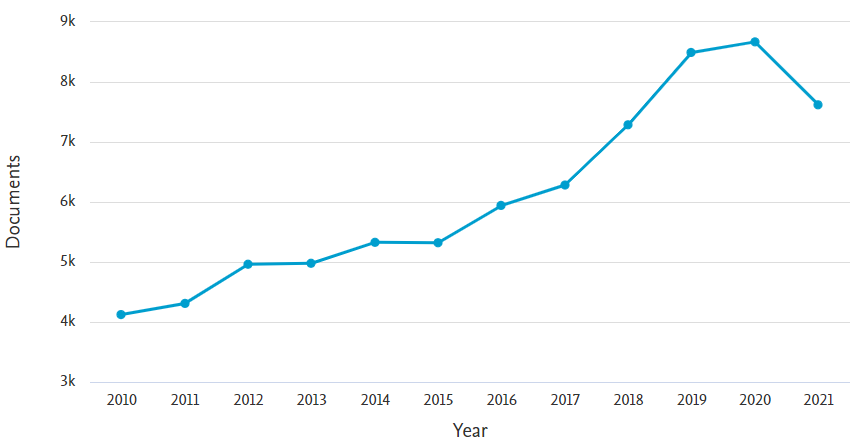
\includegraphics[scale=0.5]{"Part 2 - Search-Based Optimization/Particle Swarm Optimization/Images/PSO Year.PNG"}
  %%\vspace*{-.4cm}
  \caption{Number of articles per year of PSO between 2010 and 2021. \label{fig:PSOyear}}
  %\vspace*{-.3cm}
\end{figure}


%The modifications of PSO are also part of this case in the computer science or engineering field. 
To graphically show where the PSO impacts in the last ten years Fig.~\ref{fig:PSOarea}  presents a pie chart. The main field of application is engineering, followed by computer sciences, and third place in mathematics.

\begin{figure}[h!]
  %\vspace*{-.2cm}
  \centering
  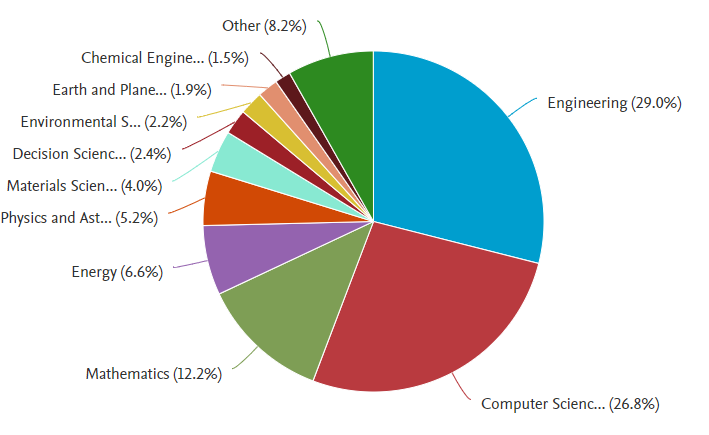
\includegraphics[scale=0.5]{"Part 2 - Search-Based Optimization/Particle Swarm Optimization/Images/PSO Area.PNG"}
  %%\vspace*{-.4cm}
  \caption{Documents by subject area related to PSO between 2010 and 2021. \label{fig:PSOarea}}
  %\vspace*{-.3cm}
\end{figure}

In this chapter, an introduction to the PSO algorithm is given. The goal is to provide an overview of the PSO, explain its basic concepts and operators, and present examples and exercises. Besides, the variants of the PSO are also discussed based on their importance in the scientific community. In the same context, they also studied the most important application of this vital algorithm.

The rest of the chapter is organized as follows: Section \ref{sec:psobasics} explains the operators of the PSO. Section \ref{sec:variants} discusses the main modification of the PSO. In Section \ref{sec:apps} are analyzed the most important PSO applications. Finally, Section \ref{sec:conclusions} discuses some conclusions and proposes some exercises.
%\todo[inline]{ DIEGO}
%Supervised learning: consider a set of examples 

%\[\mathcal{T} = \{(\mathbf{x}^{(1)},y^{(1)}),(\mathbf{x}^{(2)},y^{(2)}),\cdots,(\mathbf{x}^{(N)},y^{(N)})\}\]

%\noindent where $(\mathbf{x}^{(i)},y^{(i)}) \in \mathcal{X} \times \mathcal{Y}$  are drawn i.i.d. (independently and identically distributed) from a fixed albeit unknown joint probability distribution $p(\mathbf{x},y)$.

%Supervised learning aims at building a (predictive) model able to generalise to unseen (test) examples of the same probability distribution $p(\mathbf{x},y)$. In classification problems, $\mathcal{Y}$ is a set of categories / classes. In regression problems, $\mathcal{Y}$ is $\mathbb{R}$.

%Supervised learning aims at learn a (predictive) model able to generalise to unseen (test) examples of the same probability distribution% $p(\mathbf{x},y)$. In classification problems, $\mathcal{Y}$ %is a set of categories / classes. In regression problems, $\mathcal{Y}$ is $\mathbb{​R}$.


%Mathematical notations:
%\begin{itemize}
%\item Scalar: lower case, e.g., $a$, $b$.
%\item Column vector: lower case, bold, e.g., $\textbf{x}$.
%\item Vector element: lower case with subscript, e.g., $x_1$, $x_2$.
%\item Matrix: upper case, bold, e.g., $\textbf{X}$.
%\item Matrix element: upper case with subscripts, e.g., $X_{1,2}$.
%\item If enumerating these (e.g., having multiple vectors), superscript will be used to differentiate this from indices, e.g., $\textbf{x}^{(1)}$, $\textbf{x}^{(2)}$.
%\item Use mathcal font for sets, e.g., $\mathcal{T}$ for training set.
%\end{itemize}

%Terms to be adopted:
%\begin{itemize}
%\item Please use the term ``input variable'' instead of ``independent variable'' or ``input attribute''.
%\item Please use the term ``output variable'' instead of ``dependent variable'' or ``output attribute''.
%\item Please use the term ``example'' instead of ``observation'', ``data point'' or ``instance''.
%\end{itemize}
 

%\newpage
\section{The fundamentals of PSO algorithm}
\label{sec:psobasics}

This section introduces the basic concepts of the standard PSO and how it works. The pseudocode is described easily, and an example permits an analysis of the behavior of the algorithm.

\subsection{The PSO structure}

Essentially, each particle in the swarm (which is considered a candidate solution) is randomly distributed and represented by a vector in a multidimensional search space; all this set of particles is considered the initial population. Once established the initial population, PSO searches for optima by updating each particle according to notions such as position, velocity, inertia, etc. These notions can be defined as a vector usually called \textit{the velocity vector}, which helps to determine the next movement of the particle. Nonetheless, this movement is not entirely random; each particle is attracted towards both its own personal best position and the best position of the swarm. Then, the population is evaluated in the objective function to determine the population quality. This also allows finding the best element that will be defined as a criterion to beat in the subsequent evaluation. The new generated positions of the particles and the speed with which they are moving are calculated considering the value of the best global element and the actual value of every particle compared with a random number \cite{erick2021matlab}.\\

When the population is initialized and evaluated, the particle with the lowest or highest objective value is obtained depending on whether it is a minimization or maximization problem, respectively. This found particle is called \textit{the global particle} $gB$. On the other hand, in each iteration of the algorithm, the current particle is compared with the newly generated particle; in other words, particles have to be evaluated in the objective function every time they are moved. If the generated particle is better than the current one, then it is replaced by the new particle, receiving the usual name of \textit{the actual best particle} $lB$. The general pseudocode of the particle swarm optimization algorithm is shown in Algorithm~\ref{alg:PSO}. In contrast, the phases of initialization and movement of particles that compose the PSO are explained in the following two subsections.\\

In order to better understand the pseudocode shown in Algorithm~\ref{alg:PSO}, it is enough to appreciate that it is divided into two main parts, the unnumbered part and the numbered part. The unnumbered part refers to those terms that the algorithm requires in order to perform its operation, terms such as the population number, dimensions, etc. Once the previous points have been established, the numbered part is given, which begins with the initialization of the population and its respective evaluation. The terms "repeat" and "until" refer to the beginning and end of the while loop, which is the main body of the algorithm.

\begin{algorithm}[h!]
\caption{Particle swarm optimization pseudocode}
Parameters $\rightarrow$ Dimensions, Bounds, Maximum iteration number, Number of particles.\\
Output $\rightarrow gB$.   
\begin{algorithmic}[1]
\STATE{Initialize the particles of population.}
\STATE{Evaluate the objective function.}
\REPEAT
\FOR{All particles in all dimensions}

\STATE Generate a new velocity.
\STATE Calculate a new position.
\STATE Evaluate again the objective function.
\ENDFOR
		
\STATE Update the best particle of population.
\UNTIL the maximum number of iterations is reached.
\end{algorithmic}
\label{alg:PSO}
\end{algorithm}

\subsubsection{Initialization of the PSO}

All meta-heuristic algorithms have an initialization phase that has the primary purpose of creating the initial population, where each particle represents a candidate solution for the optimization problem. These particles are randomly generated in a search space, which is delimited by the established bounds. Generally, the initialization phase also defines the parameters of the problem to optimize \cite{erick2021matlab}. The initialization of the PSO algorithm is defined by Eq.~\ref{eq:equation1}, which describes the optimization of its individual particles.

\begin{equation}
\vec{x}_{i,j}^t=lb_j+rand(ub_j-lb_j)
\label{eq:equation1}
\end{equation}

Where, $\vec{x}_{i,j}^t$ is the $i-th$ population particle, $i$ represents the index of a given particle and its size is $(i=1,2,3,...,N)$, where $N$ is the maximum number of particles, $j$ represents the $j_{th}$ dimension of the design variable understanding that $0<j\leq d,$ where $d$ is the dimensionality of the design variable. The iteration number is represented by $t$. While $lb_j$ and $ub_j$ define the lowest and upper limit, respectively. It is worth saying that $rand$ is a uniformly distributed random number between $0$ and $1$. Once established the respective position of each particle, it is necessary to define the velocity each one of them will move around the search space to find the global optimal. We will explain that phase next.

\subsubsection{Velocity and movement of particles}

To find the velocity, it is necessary to get the best global and local values of each particle, commonly called $\vec{gB}^t$ and $\vec{lB}_i^t$ respectively. Eq.~\ref{eq:equation2} defines the velocity calculation for each particle $i$.

\begin{equation}
\vec{v}_i^{t+1}=w \times \vec{v}_i^{t}+c_{1} \times \vec{r1}^t \times (\vec{lB}_i^t-\vec{x}^{t}_i)+c_{2} \times \vec{r2}^t \times (\vec{gB}^t-\vec{x}^{t}_i)
\label{eq:equation2}
\end{equation}

\begin{equation}
\vec{x}_i^{t+1}=\vec{x}_i^{t}+\vec{v}_i^{t+1}
\label{eq:equation3}
\end{equation}

Where $\vec{v}_i^{t+1}$ is the particle $i$'s velocity of the iteration $t+1$, $\vec{v}_i^{t}$ is the particle $i$'s velocity in the previous iteration, the vector that contains each particle $i$'s position is $\vec{x}_i^{t}$ and $\vec{r1}^t$ and $\vec{r2}^t$ represent $d$-dimensional vectors containing uniformly distributed random numbers between $0$ and $1$. It is worth to say that $c_{1}$ and $c_{2}$ are called learning coefficients, and $w$ represents an inertia weight that affects the convergence and exploration- exploitation trade-off in PSO process. Since inception of inertia Weight in PSO, a large number of variations of Inertia Weight strategy have been proposed, nonetheless, it is generally established as 1. Meanwhile, Eq.~\ref{eq:equation3} is used to displace the particles to new positions in the next iteration. Where $\vec{x}_i^{t+1}$ is the vector where the new obtained position of particle $i$ at iteration $t+1$ is stored, $\vec{x}_i^{t}$ corresponds to the previous position of particle $i$ calculated at iteration $t$, and finally $\vec{v}_i^{t+1}$ is the velocity vector obtained by Eq.~\ref{eq:equation2}.

It is essential to mention that the majority of modifications to the PSO algorithm have as purpose to find new ways to accelerate the particles as best as possible \cite{erick2016optimizacion}. To end this section, Fig.~\ref{fig:PSOmovement} shows a graphic description of particle's velocity and their movement in the particle swarm optimization algorithm for a better understanding by the reader.\\

\begin{figure}[h!]
\centering
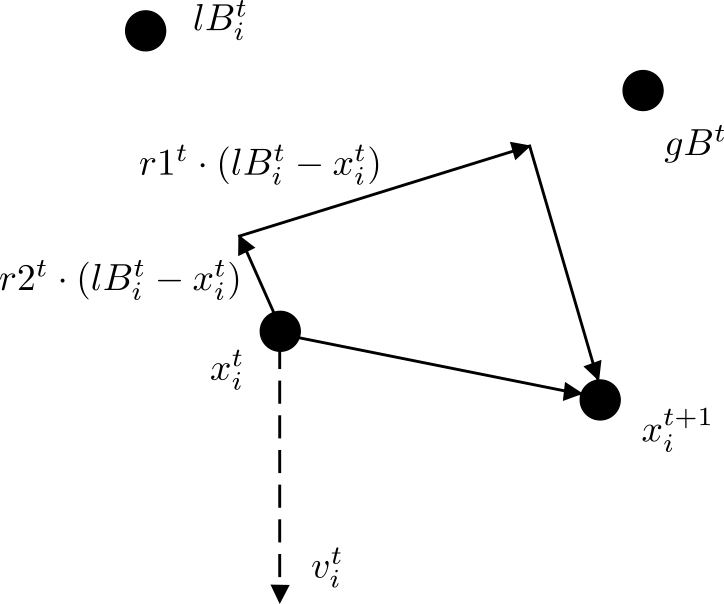
\includegraphics[scale=0.4]{"Part 2 - Search-Based Optimization/Particle Swarm Optimization/Images/Fig.1.3.png"}
\caption{Velocity and movement of particles in PSO.}
\label{fig:PSOmovement}
\end{figure}

\subsection{A PSO example}

To show how the PSO works here is presented a graphical example. Figure~\ref{fig:f1} shows the peaks function plotted in 3D with a lateral view. This function is commonly used in the literature to explain the behavior of optimization algorithms. Figure~\ref{fig:f2} shows the random initialization of the population of a particle (swarm) in PSO \cite{kennedy1995particle}. The population has 30 particles uniformly distributed in the search space defined by the peaks function with an upper bound as $ub=3$ and a lower bound as $lb=-3$ (from the top view).\\
The examples show the distribution of particles at different stages of the optimization process establishing $1000$ iterations as a stop criteria. In Figs.~\ref{fig:f3}, \ref{fig:f4}, \ref{fig:f5} and \ref{fig:f6} it is shown the interaction of the swarm in 50, 300, 600 and 999 iterations in the test function. Finally, in Fig.~\ref{fig:f6} it is possible to see that the swarm has found the zone of the global minimum according to the color bar for the z-axis of Fig.~\ref{fig:f1}.

\begin{figure}[hbp]
  \begin{subfigure}[b]{0.5\textwidth}
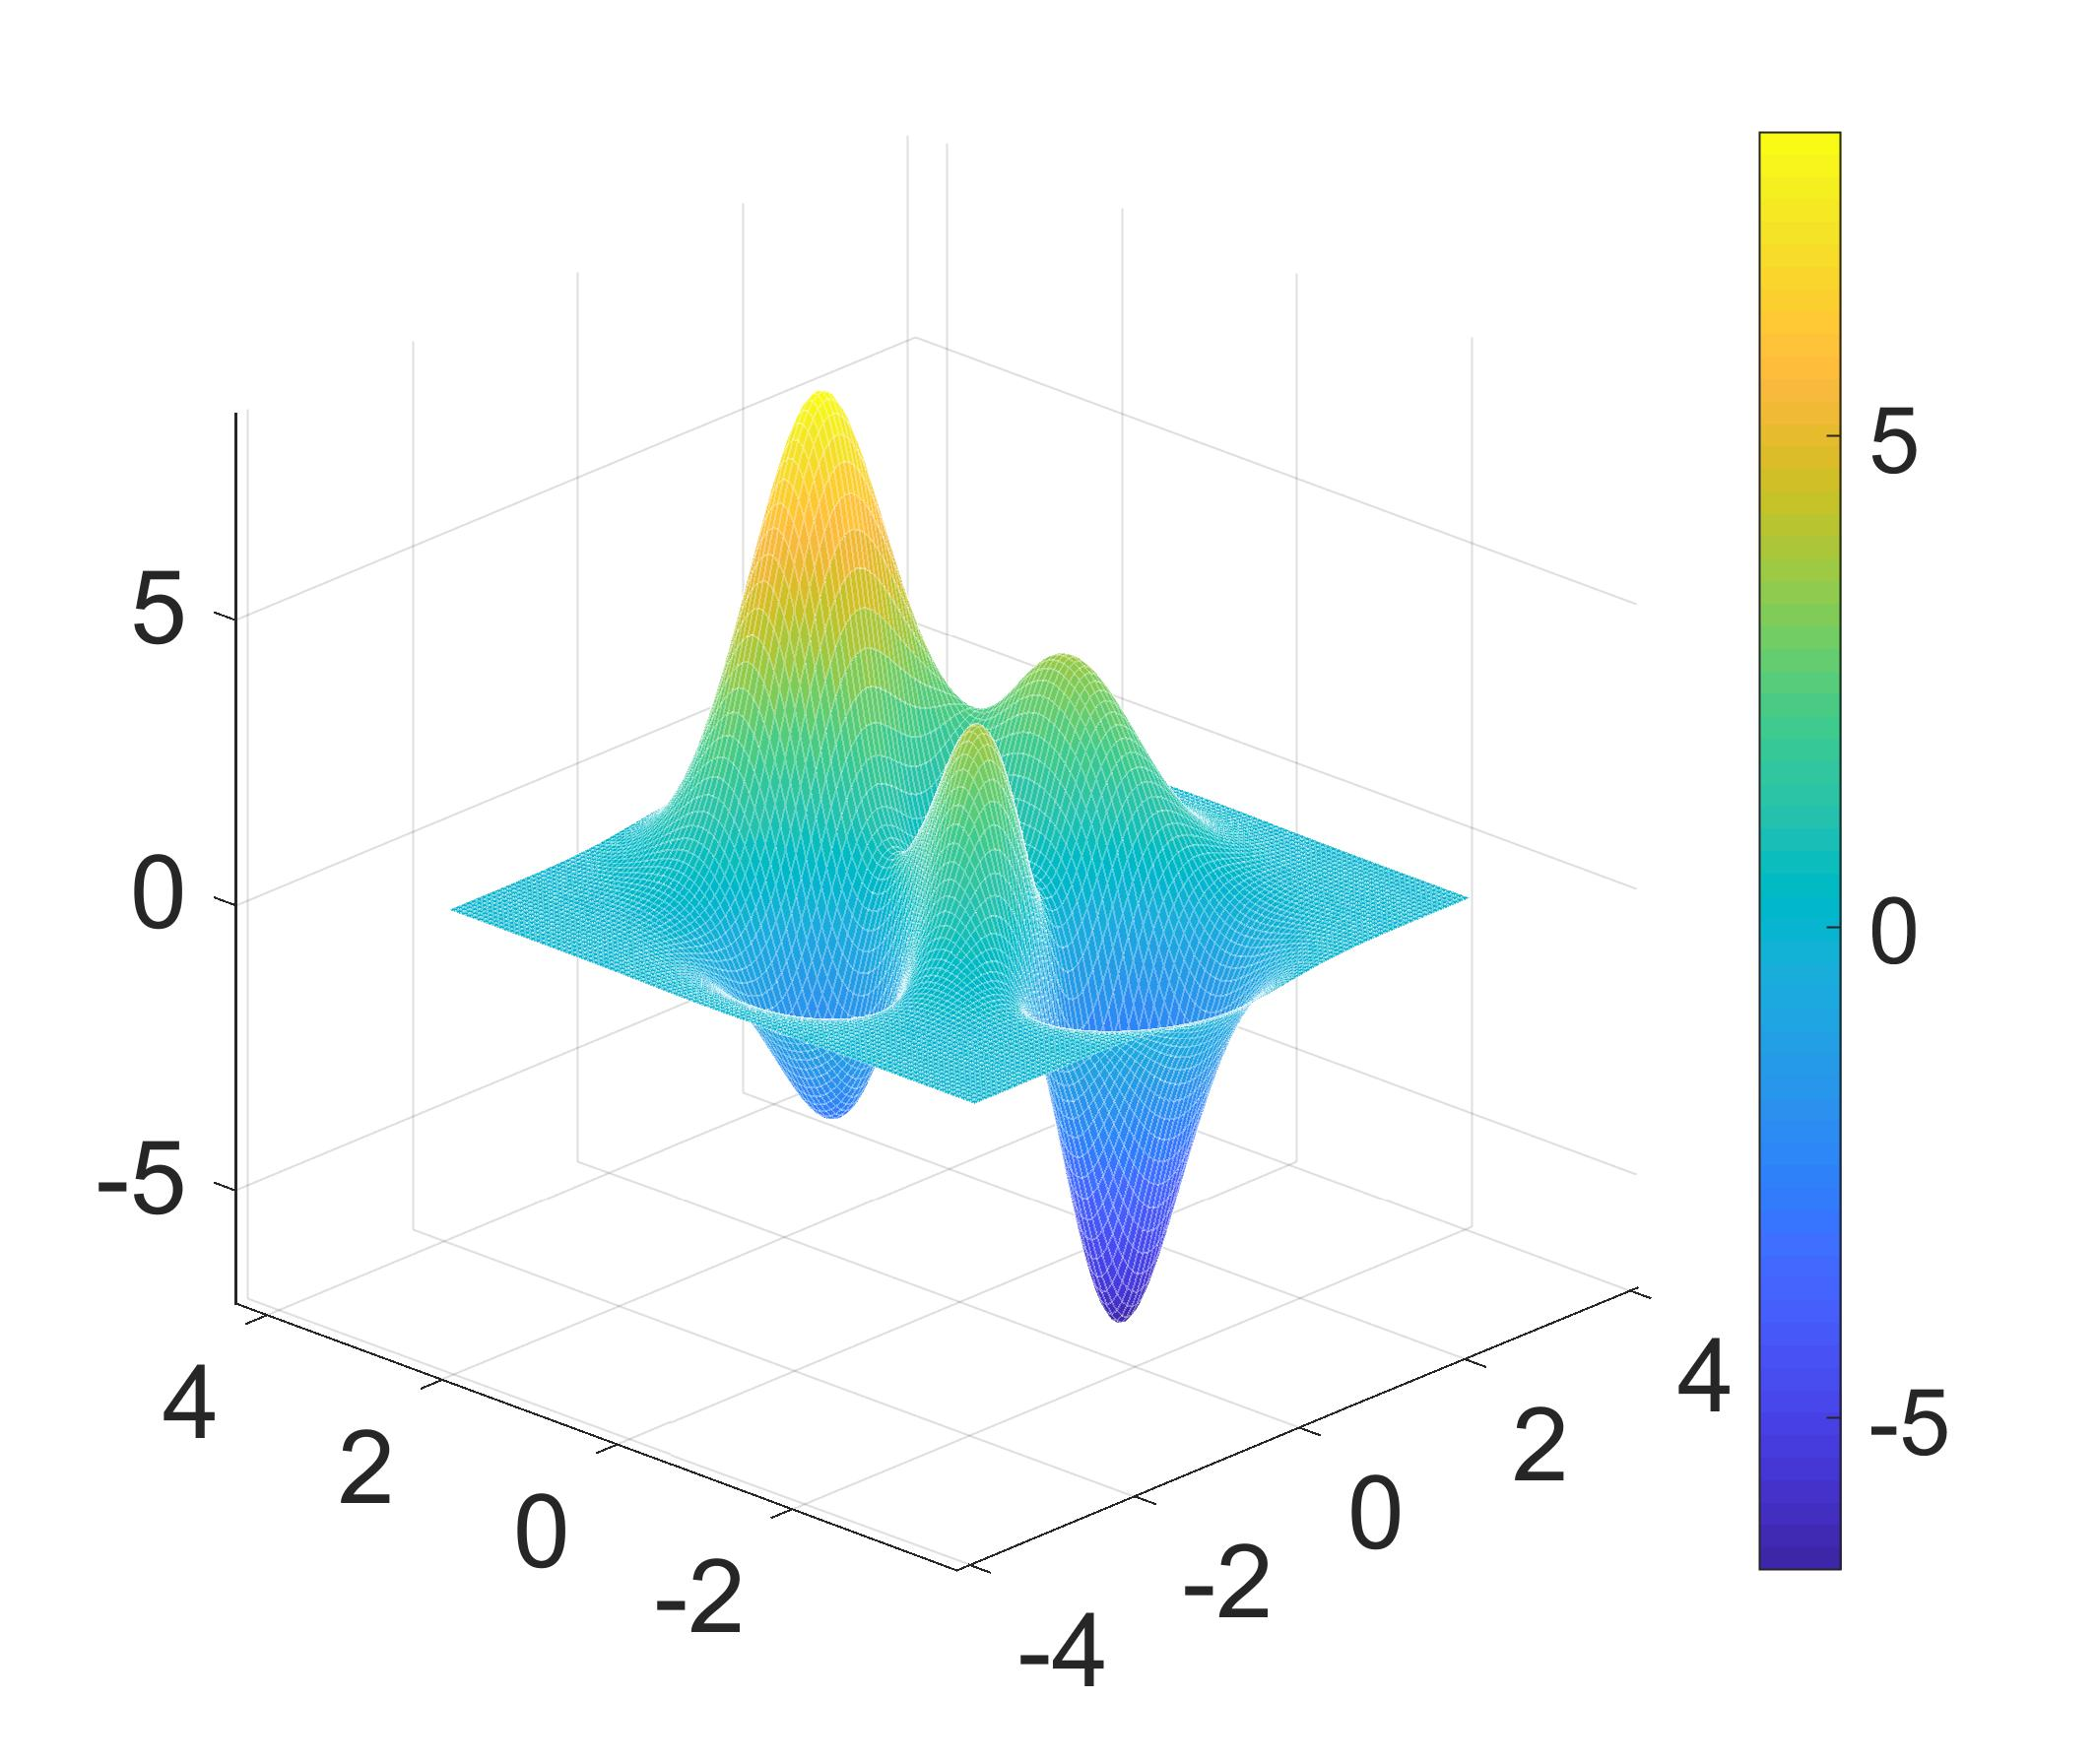
\includegraphics[width=\textwidth, height=\textwidth]{"Part 2 - Search-Based Optimization/Particle Swarm Optimization/Images/FIG1.1.jpg"}
    \caption{Peaks function.}
    \label{fig:f1}
  \end{subfigure}
  \hfill
  \begin{subfigure}[b]{0.5\textwidth}
    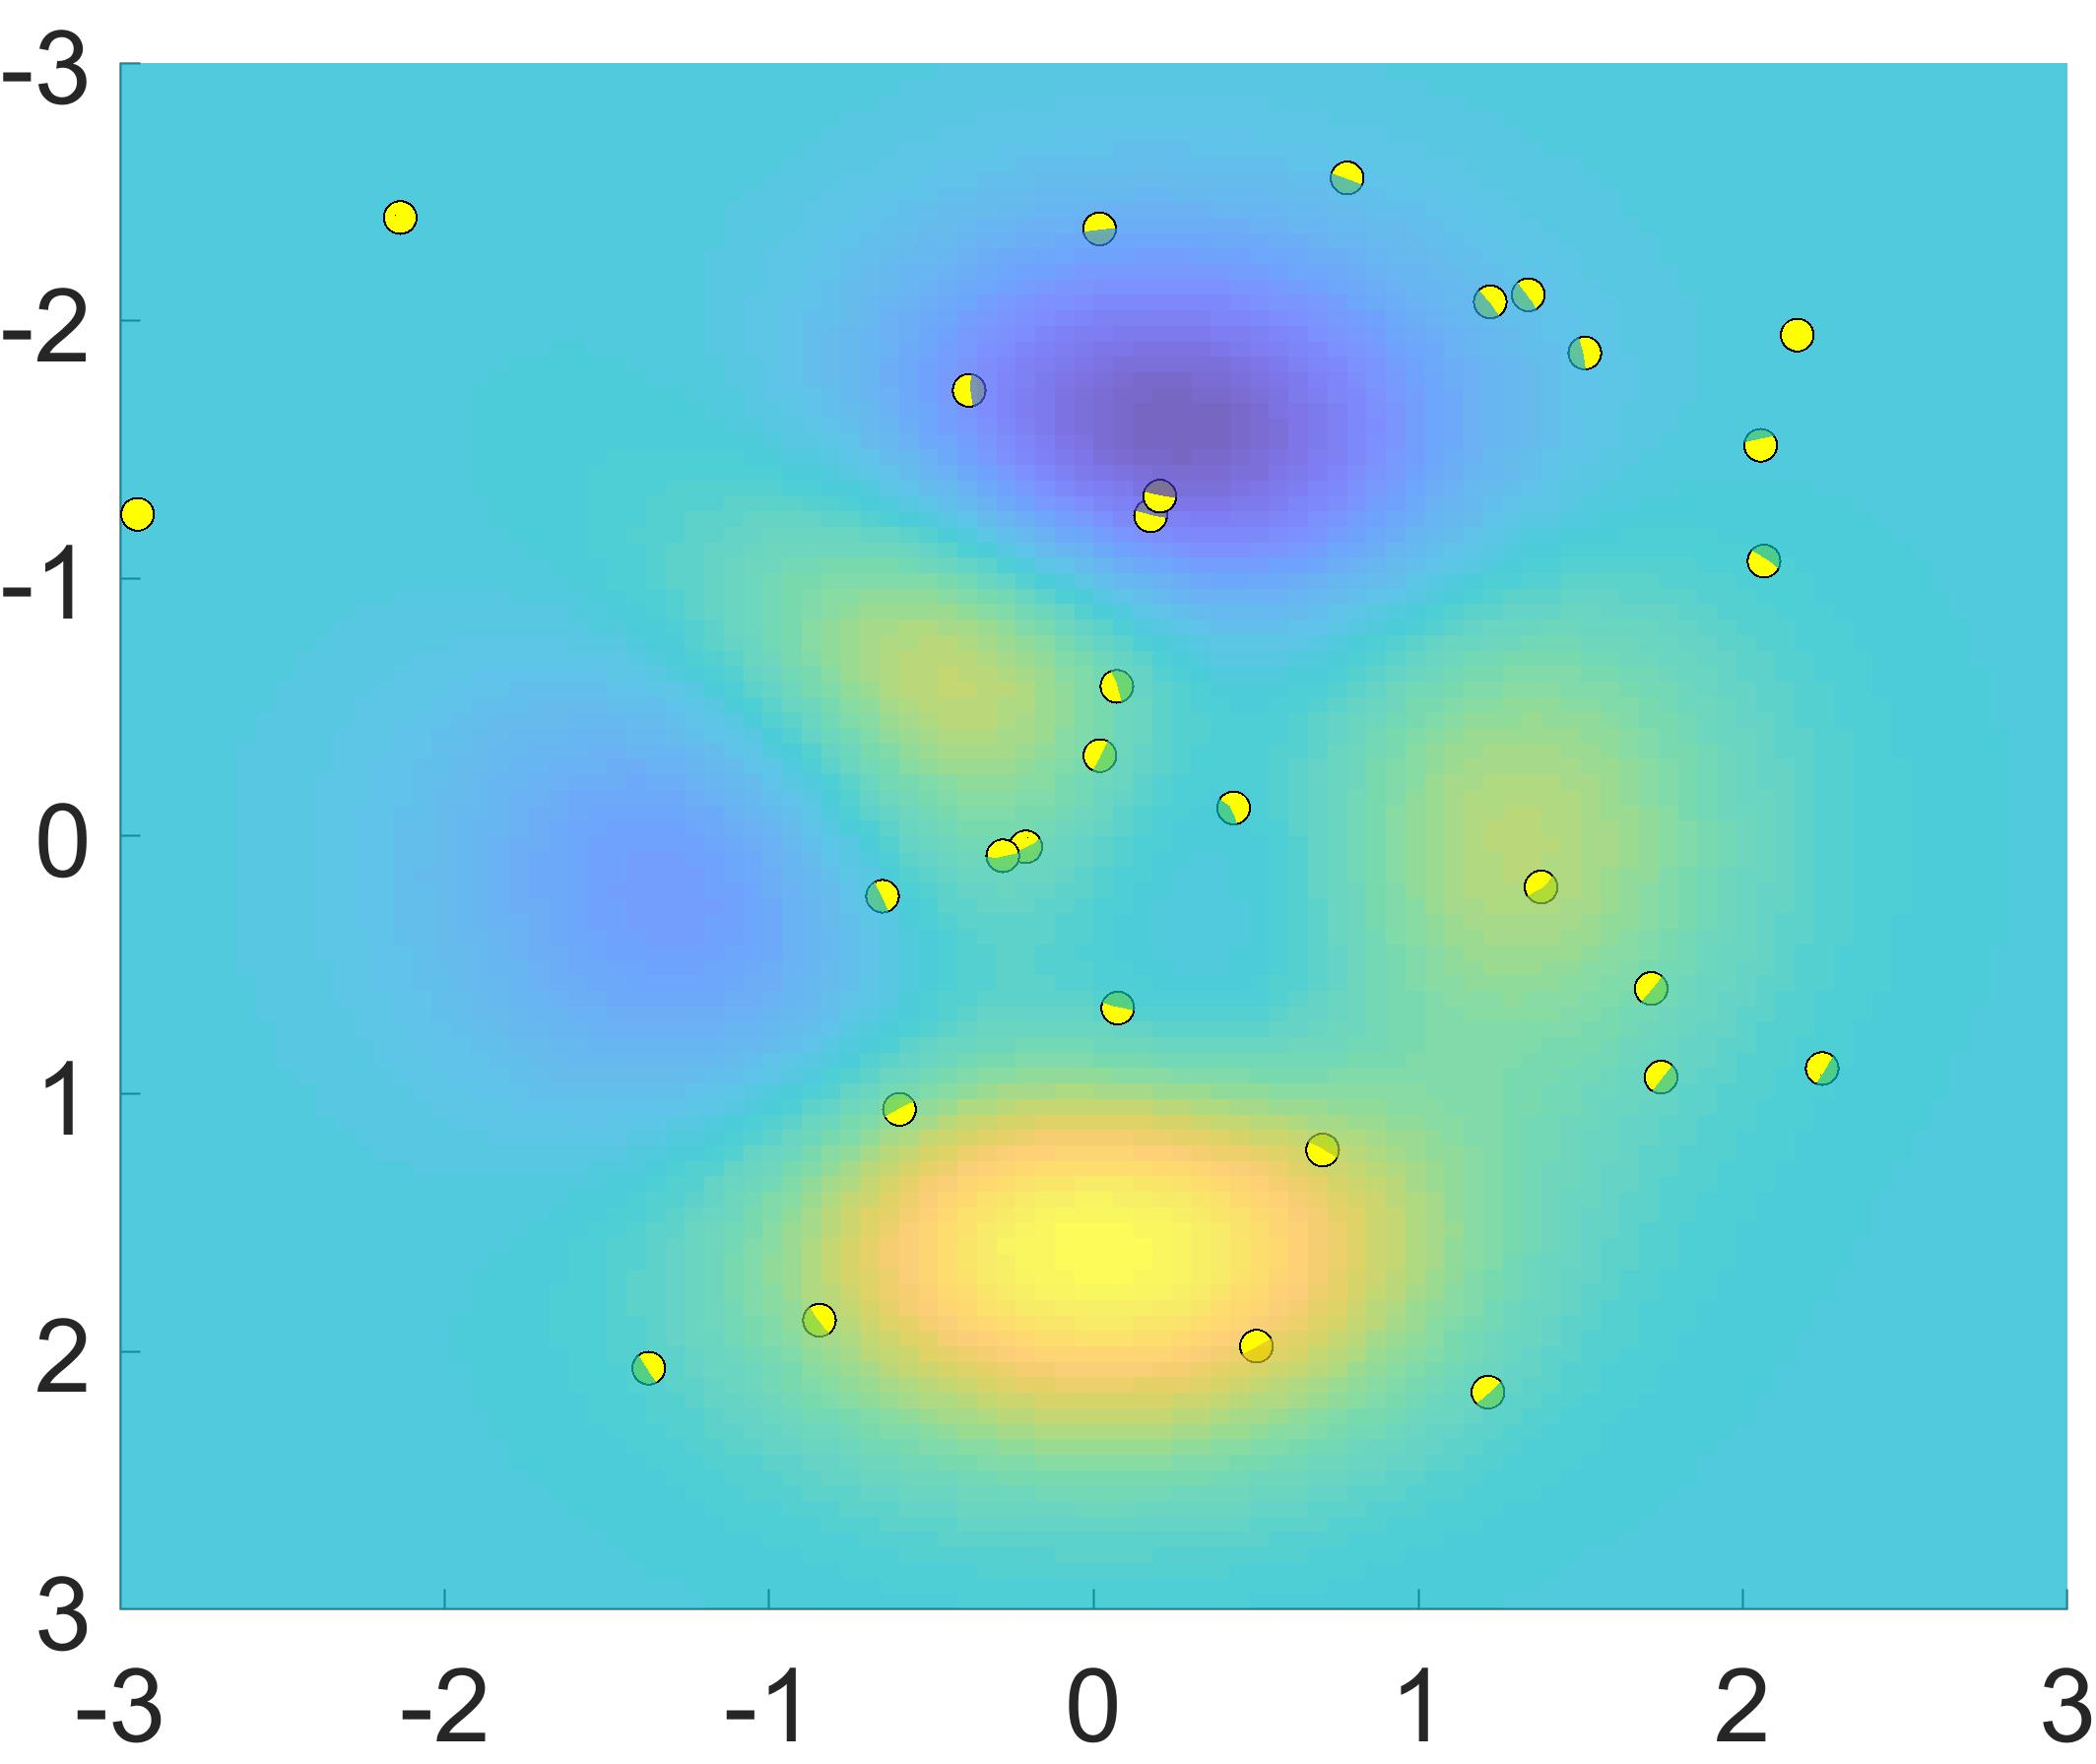
\includegraphics[width=\textwidth, height=\textwidth]{"Part 2 - Search-Based Optimization/Particle Swarm Optimization/Images/FIG2.1.jpg"}
    \caption{Distribution of the swarm at the initialization.}
    \label{fig:f2}
  \end{subfigure}
  \begin{subfigure}[b]{0.5\textwidth}
    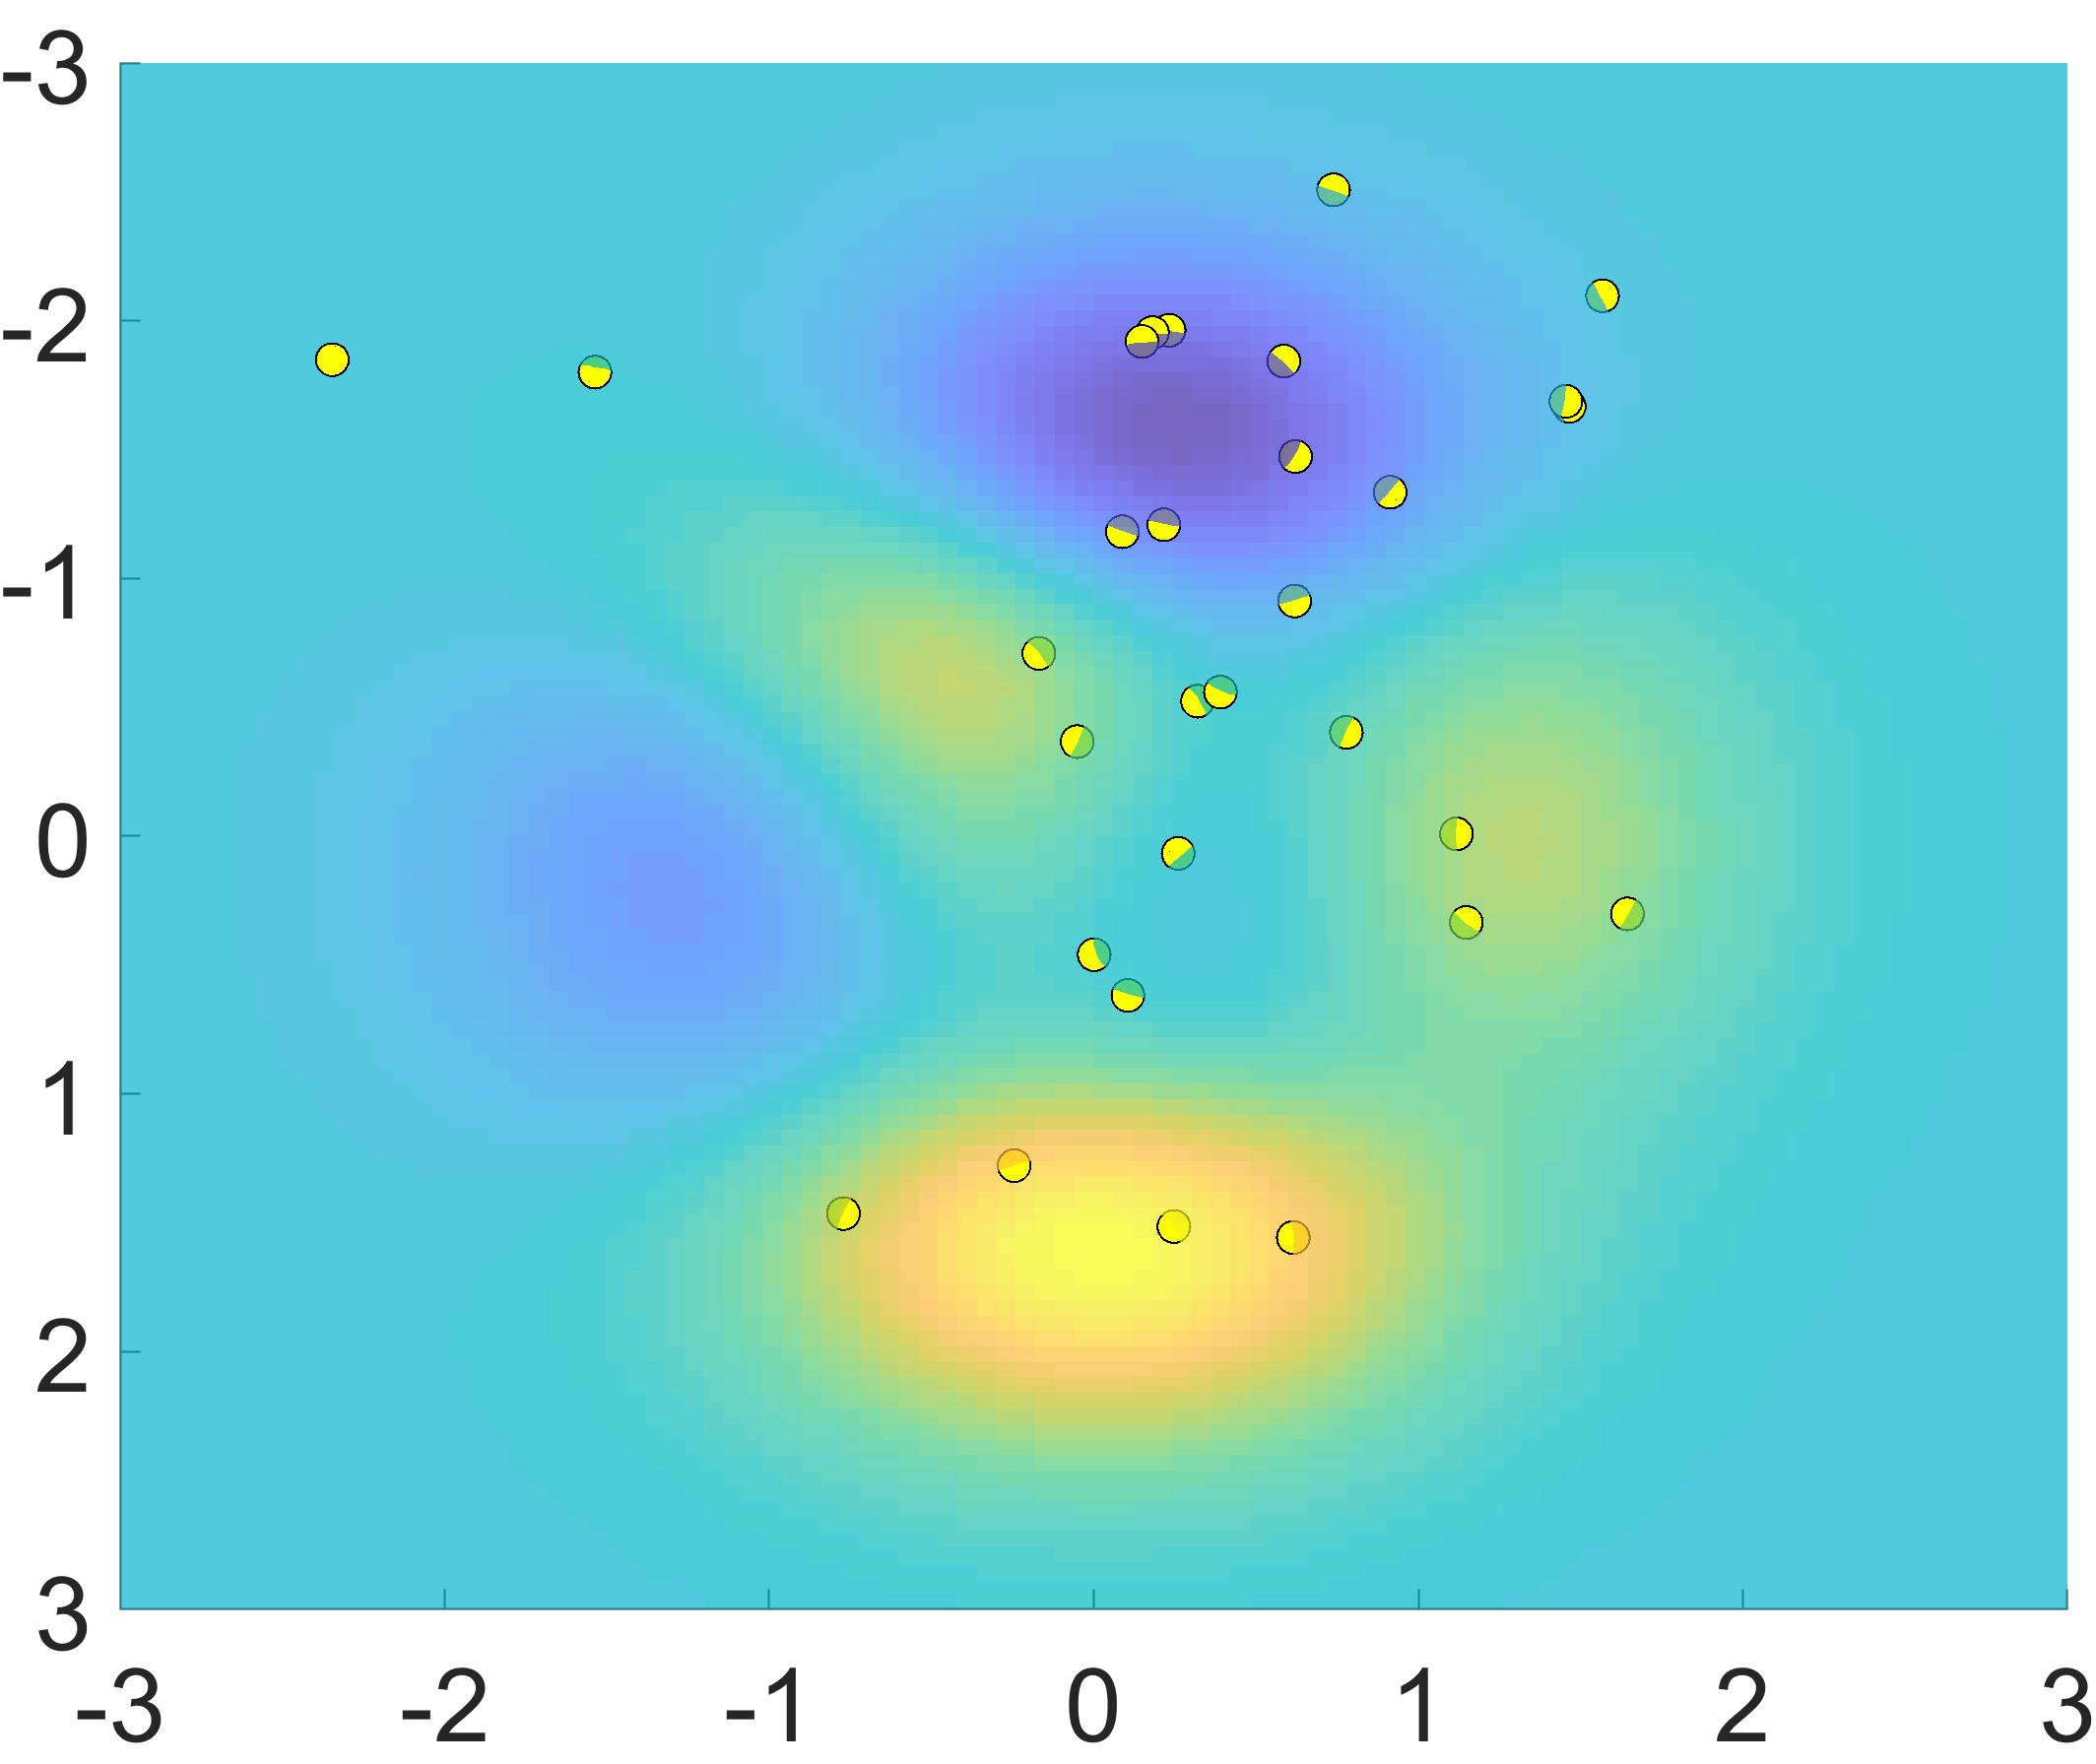
\includegraphics[width=\textwidth, height=\textwidth]{"Part 2 - Search-Based Optimization/Particle Swarm Optimization/Images/FIG3.1.jpg"}
    \caption{Distribution of the swarm at 50 iterations.}
    \label{fig:f3}
  \end{subfigure}
  \begin{subfigure}[b]{0.5\textwidth}
    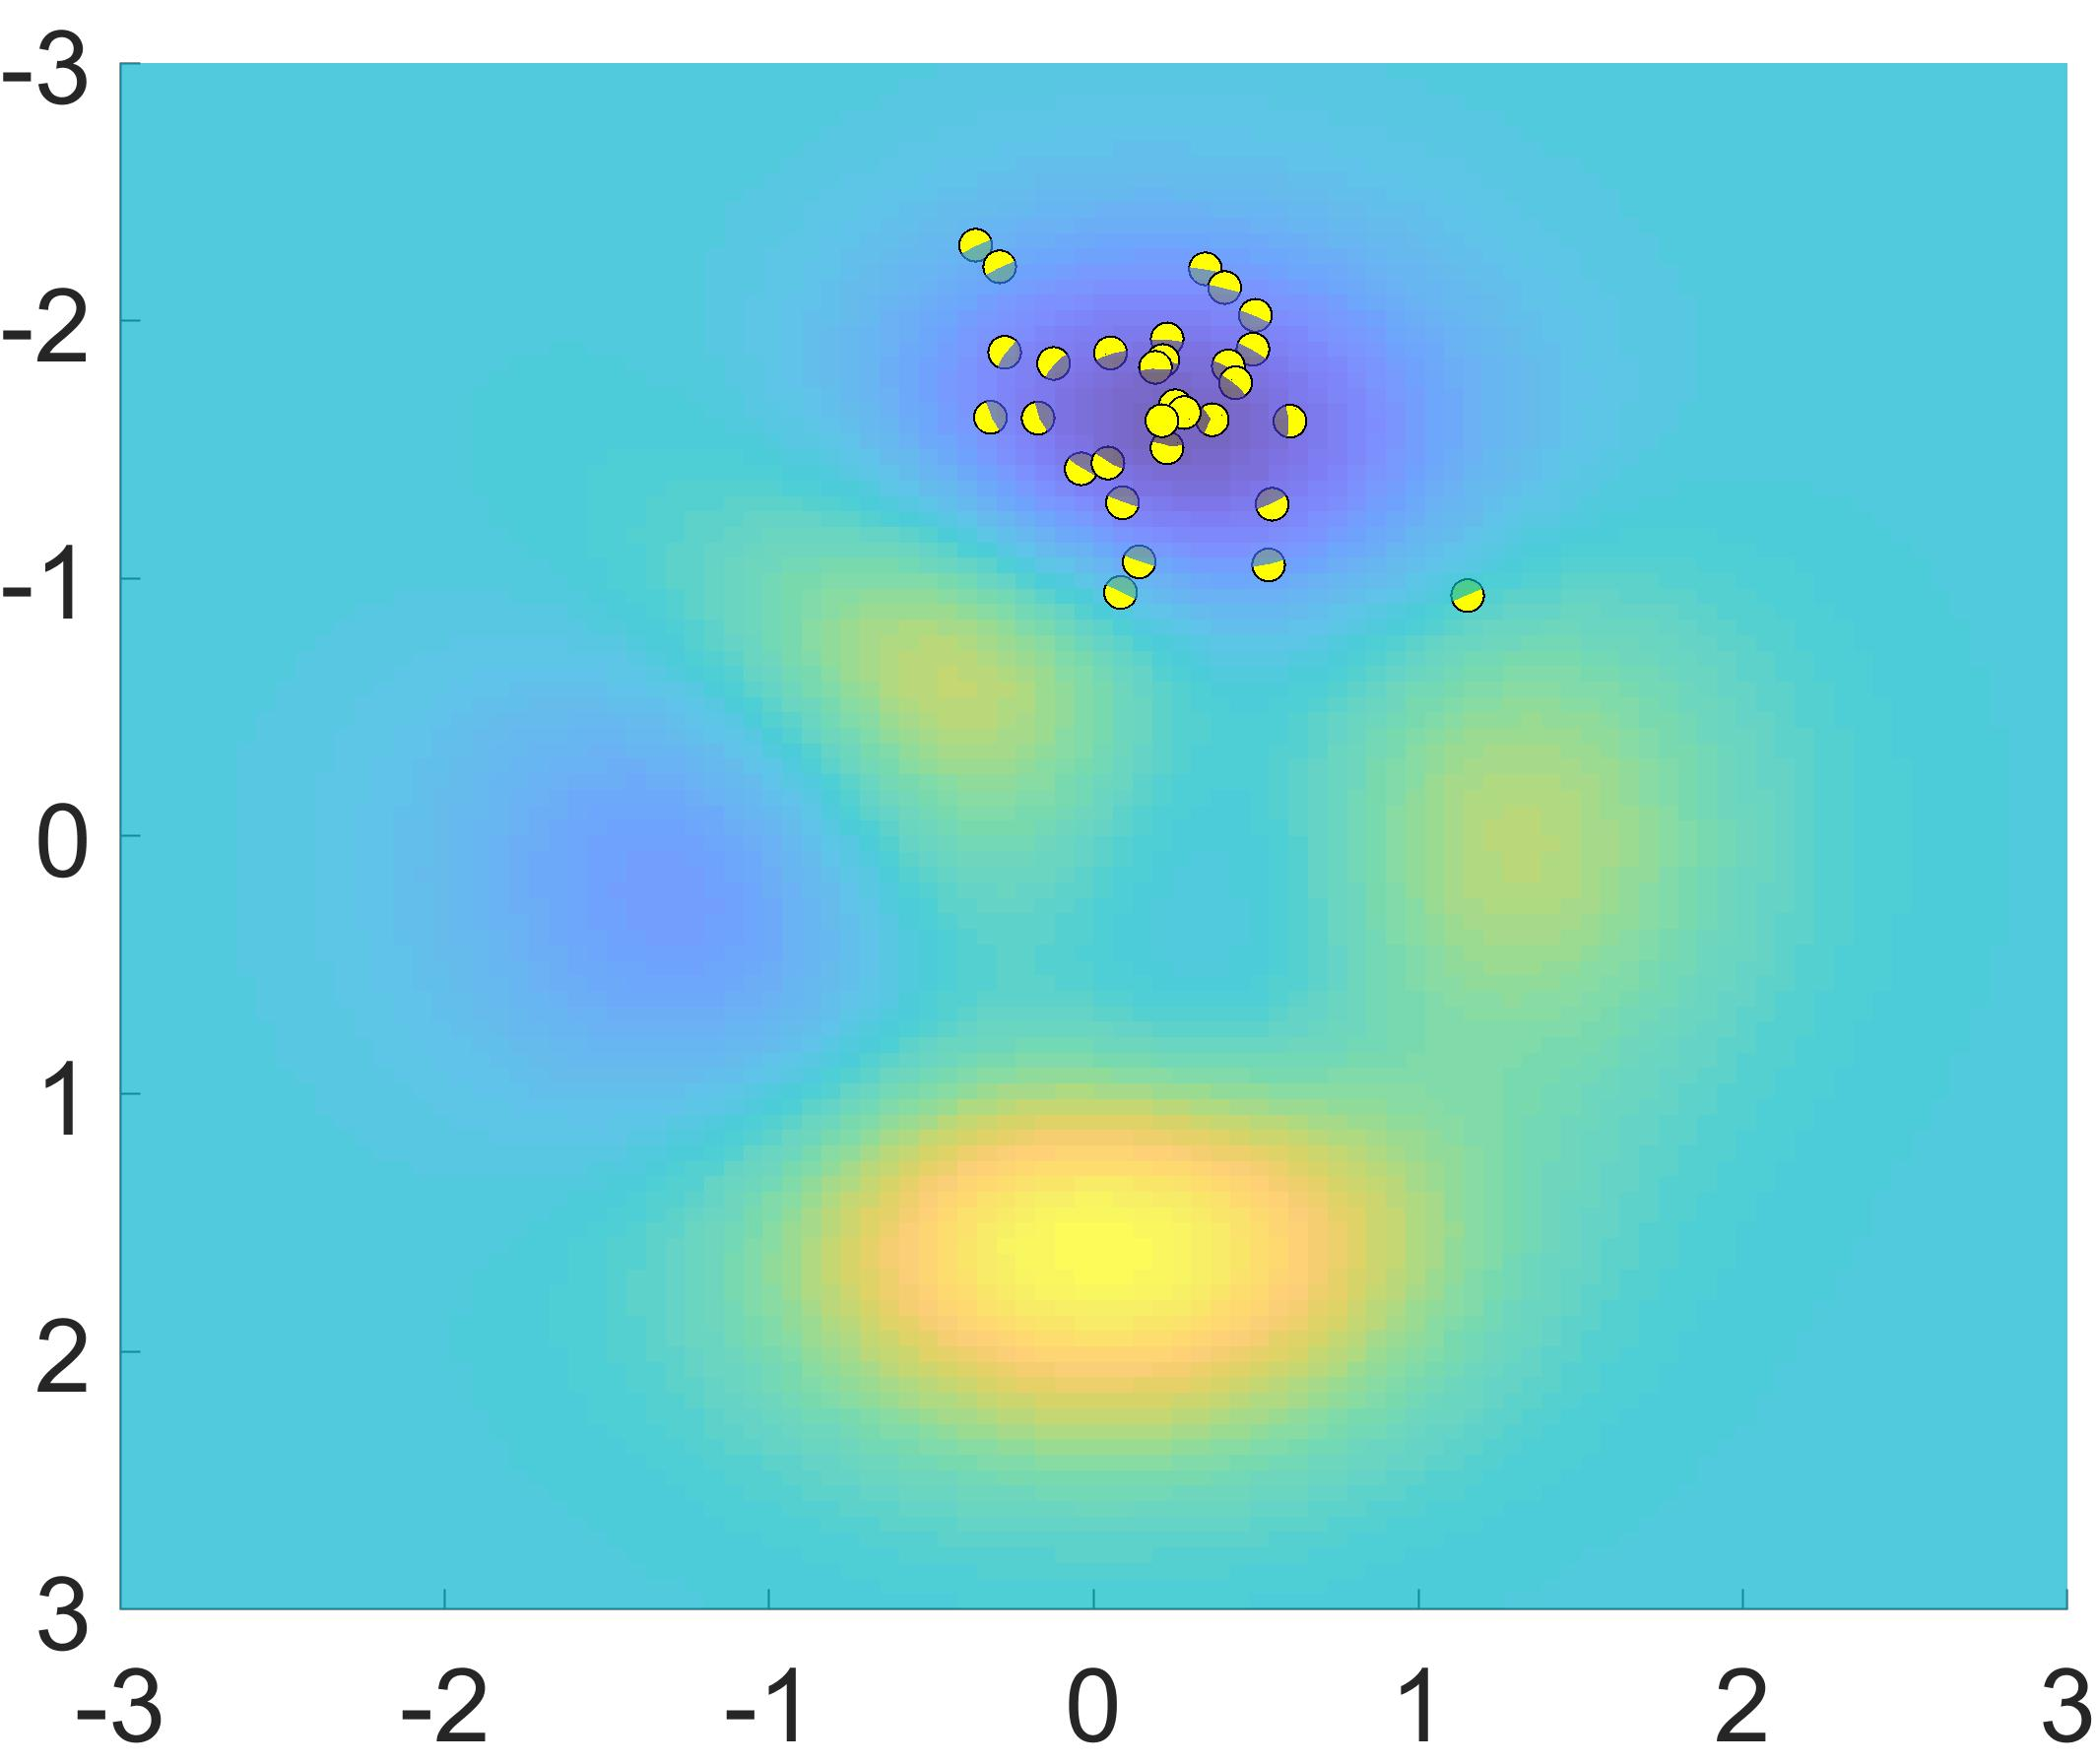
\includegraphics[width=\textwidth, height=\textwidth]{"Part 2 - Search-Based Optimization/Particle Swarm Optimization/Images/FIG4.1.jpg"}
    \caption{Distribution of the swarm at 300 iterations.}
    \label{fig:f4}
  \end{subfigure}
  \begin{subfigure}[b]{0.5\textwidth}
    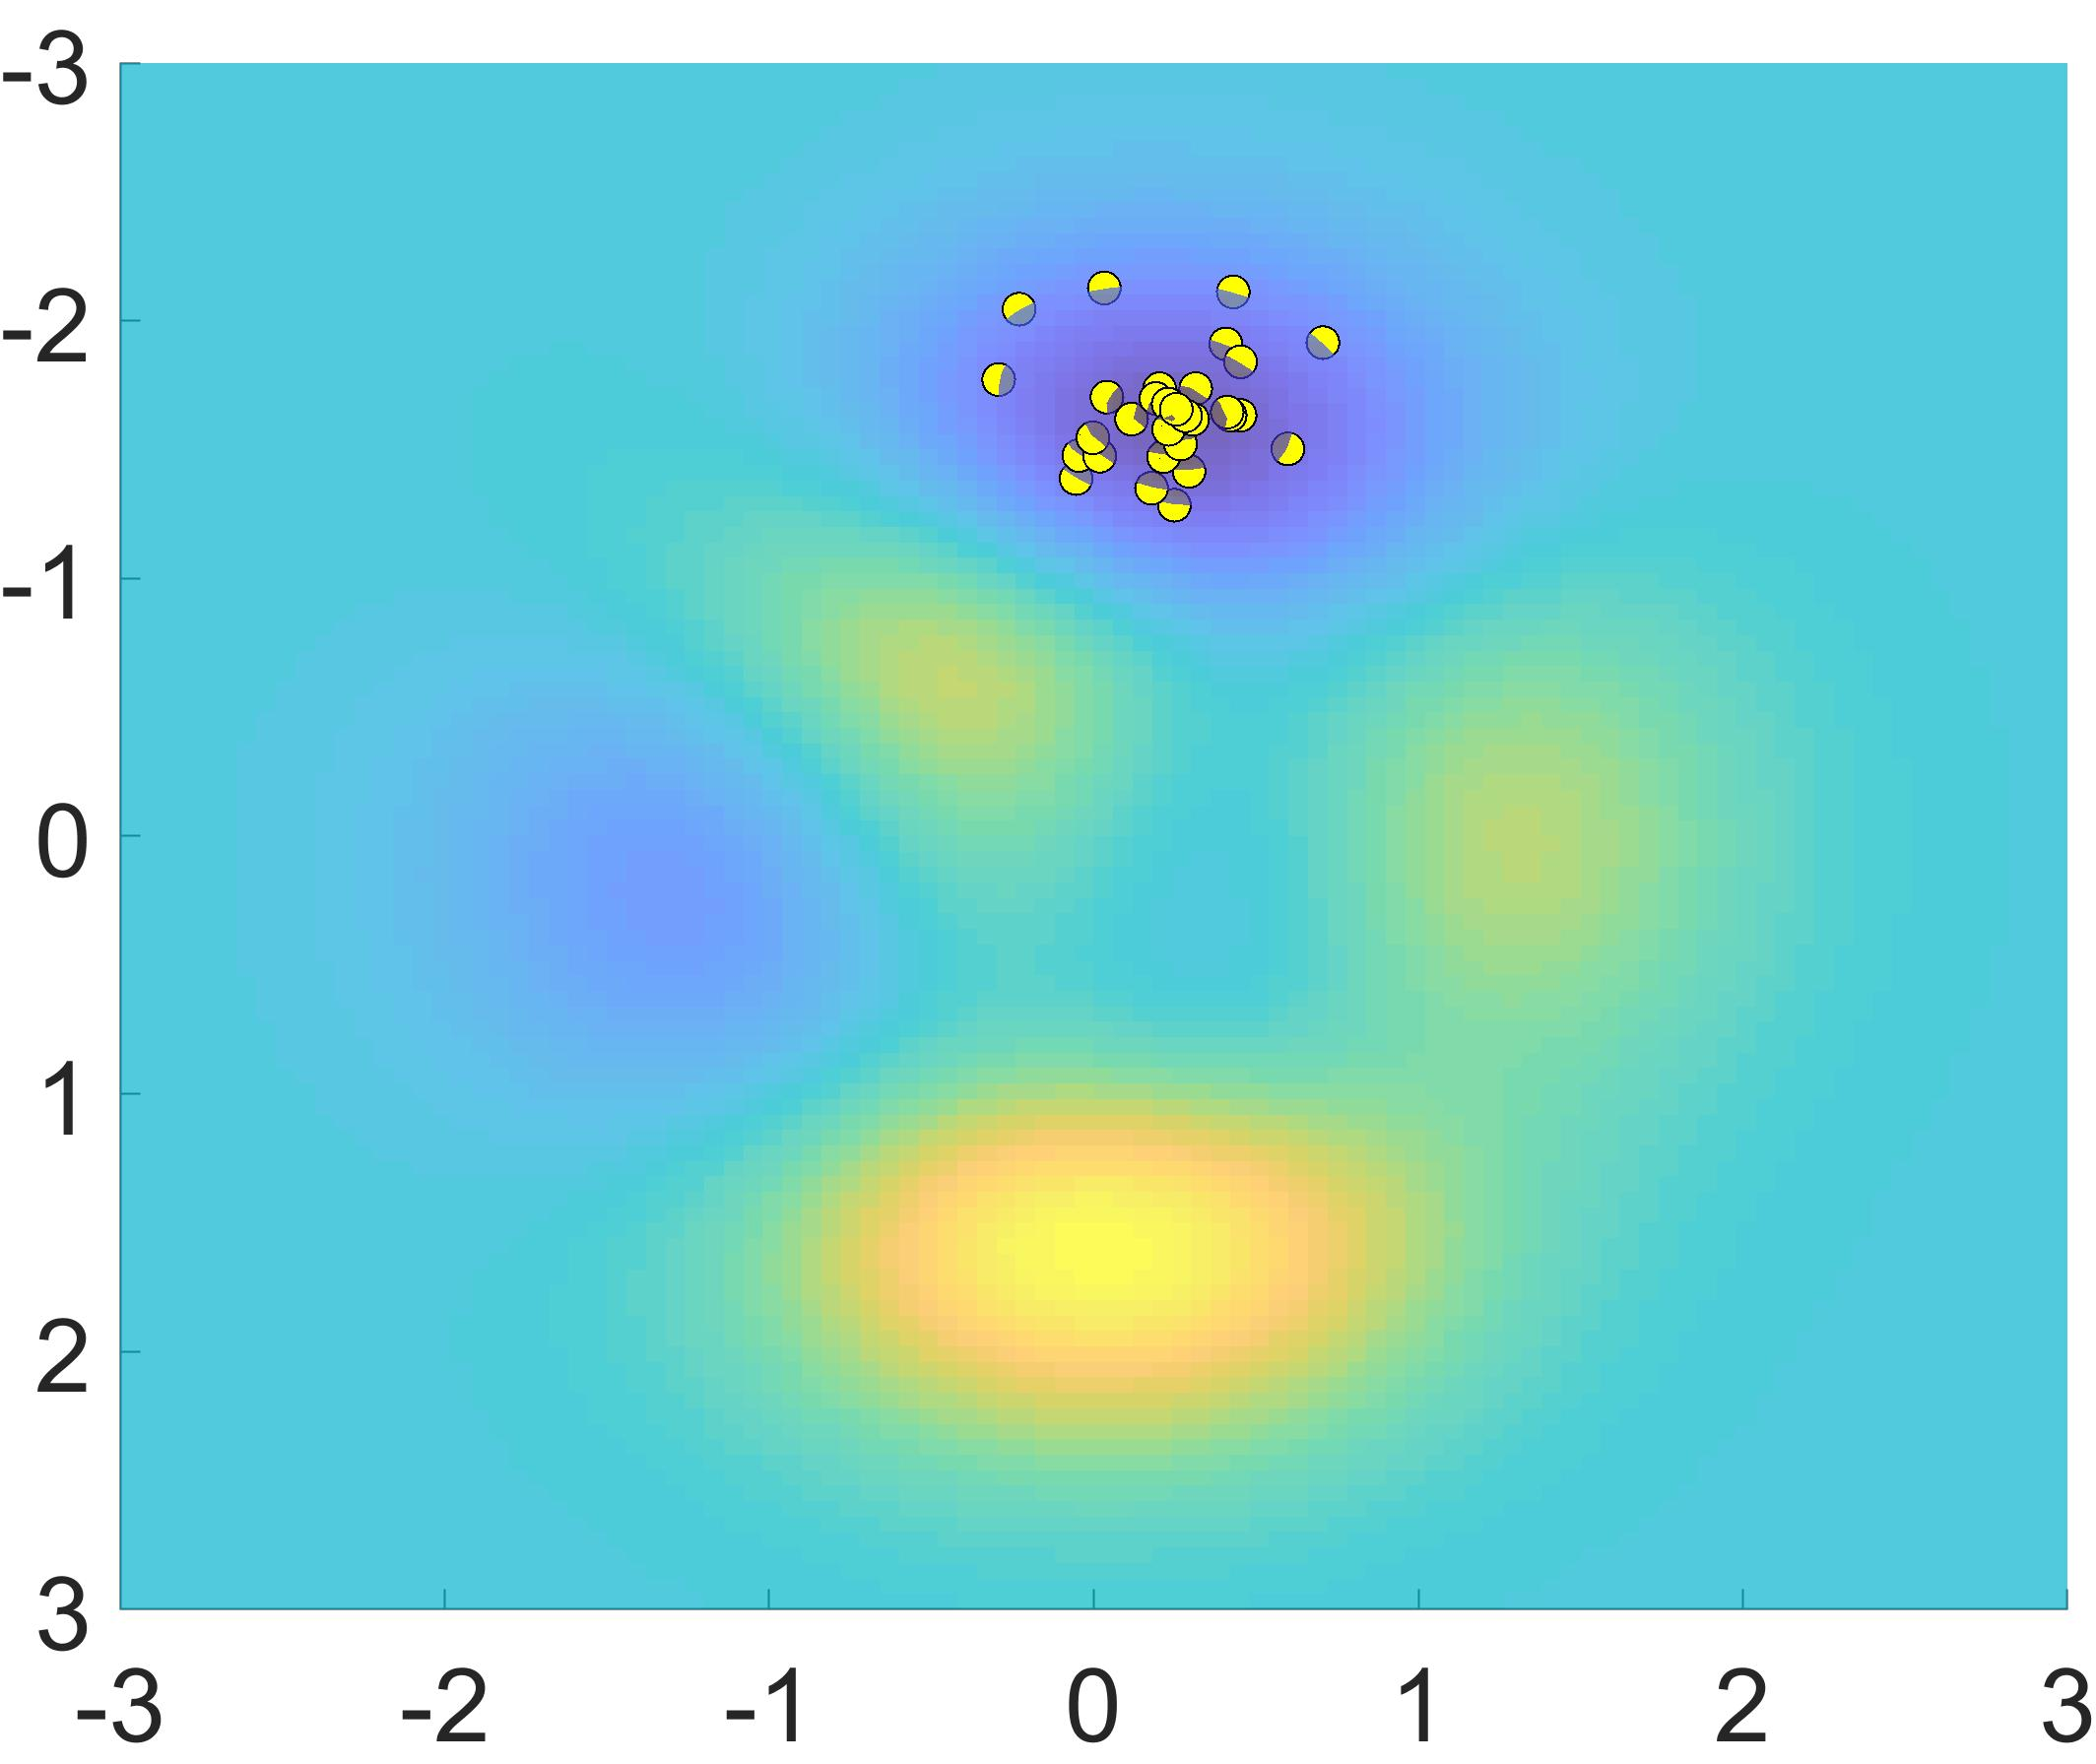
\includegraphics[width=\textwidth, height=\textwidth]{"Part 2 - Search-Based Optimization/Particle Swarm Optimization/Images/FIG5.1.jpg"}
    \caption{Distribution of the swarm at 600 iterations.}
    \label{fig:f5}
  \end{subfigure}
   \begin{subfigure}[b]{0.5\textwidth}
    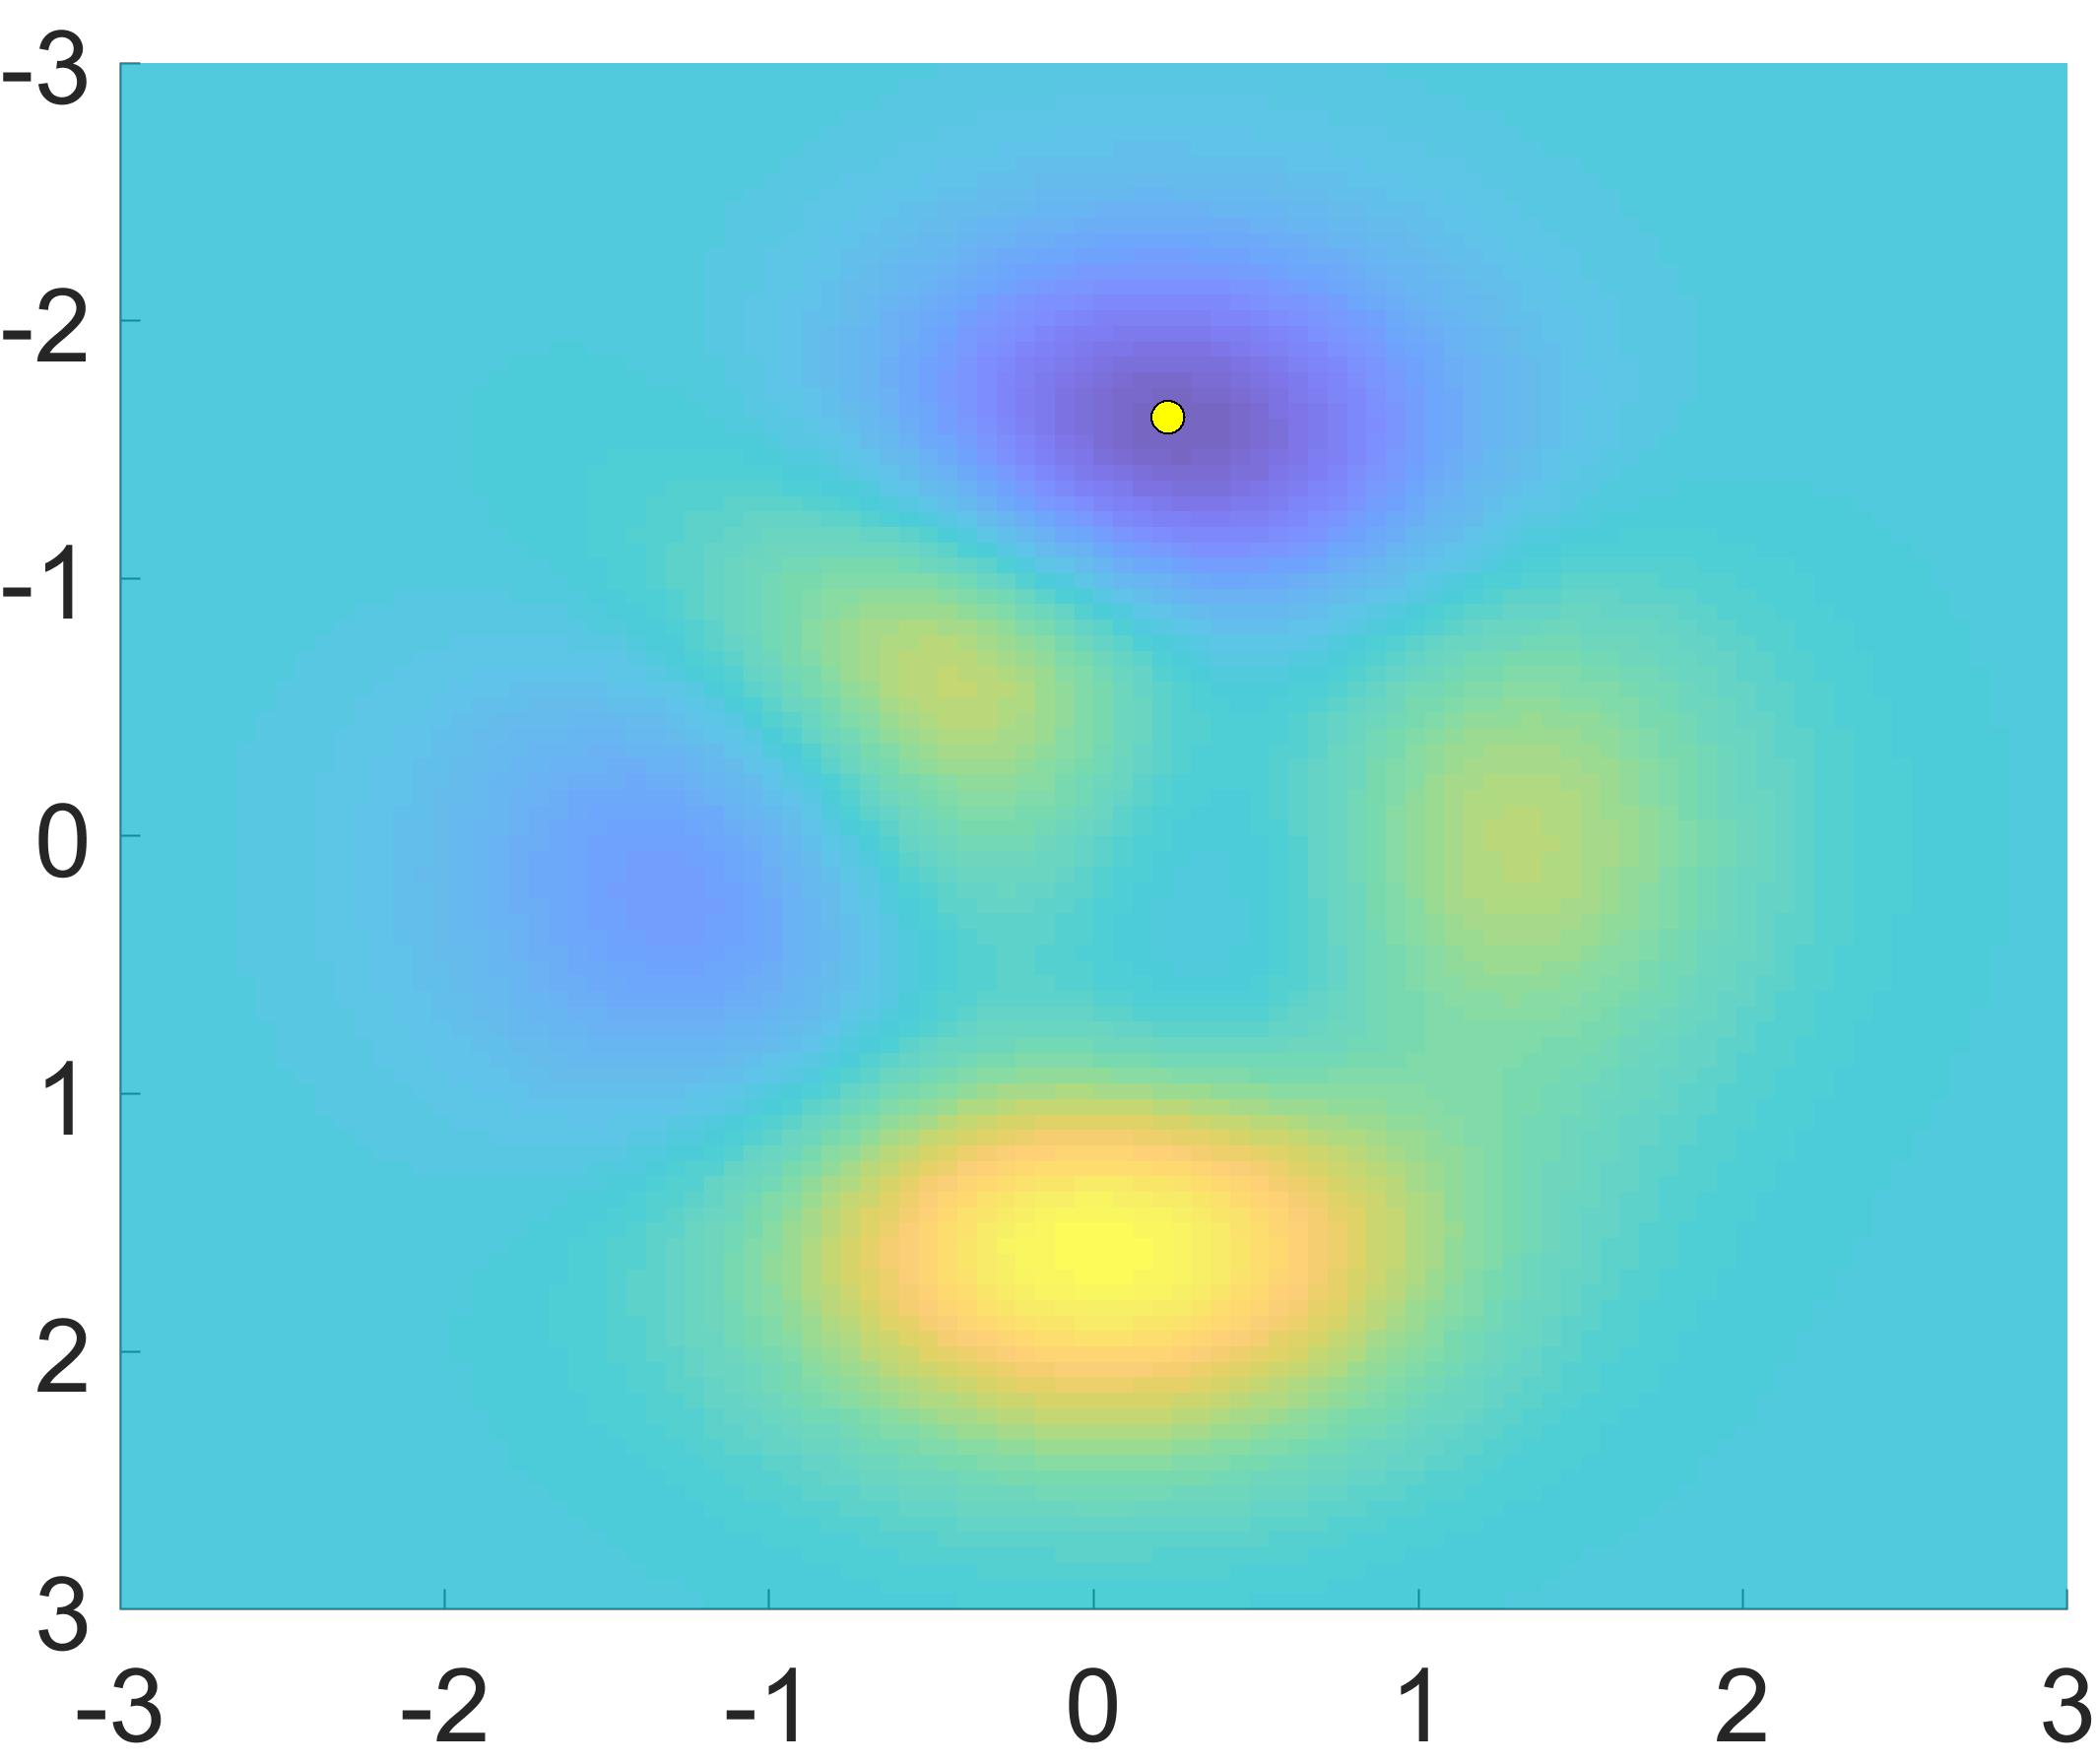
\includegraphics[width=\textwidth, height=\textwidth]{"Part 2 - Search-Based Optimization/Particle Swarm Optimization/Images/FIG8.1.jpg"}
    \caption{Final distribution of the swarm at 999 iterations.}
    \label{fig:f6}
  \end{subfigure}
  \caption{An example of the PSO along the iterative process.}
  \label{fig:fplots}
\end{figure}

%Optimization problems are problems where we want to find solutions that minimize or maximize one or more objective functions, potentially subject to certain constraints. Some examples are:

%\begin{itemize}
%\item Routing problems, e.g., to find a path from a city of origin to a city of destination that minimizes the distance travelled, while ensuring that non-existent direct paths between any two cities are not used. 
%\item Bin packing problems, e.g., to find an assignment of items to bins that minimizes the number of bins used, while ensuring that the maximum volume of the bins is not exceeded.
%\item Scheduling problems, e.g., to find an allocation of staff to tasks in a software project, so as to minimize the cost and duration of this project, while ensuring that staff are only allocated to tasks for which they have the necessary skills.
%\item Hyperparameter optimization, e.g., to find the hyperparameter values that minimize the loss (error) on the validation set for a given machine learning algorithm.
%\end{itemize}

%As we can see, in all examples above, we are interested in minimizing or maximizing a certain function (e.g., the distance travelled, the number of bins used, the cost and duration of the project and the error on the validation set). And, several these problems specify certain constraints (e.g., ensuring that non-existent direct paths are not used, ensuring that the maximum volume of the bins is not exceeded, and ensuring that staff have the necessary skills). Candidate solutions to optimization problems are referred to as \textit{feasible} if they satisfy the constraints of the problem, and \textit{infeasible} when they fail to satisfy one or more constraints.

%The examples above have been mentioned in rough terms, to give a general idea of what optimization problems are. In Section \ref{sec:formulation}, we will see what needs to be specified to formulate them more formally, so that they can be solved by optimization algorithms.


%\subsection{Optimization Algorithms}

%Optimization algorithms are algorithms that attempt to find solutions to optimization problems. They typically create one (or more) full initial candidate solutions to the problem, and then try to iteratively improve such candidate solution(s) in an attempt to find an optimal solution. This is different from search tree-based search algorithms, which attempt to systematically explore the search space to find actions that build a solution over time. 

%For example, consider a routing problem where we wish to find a path to go from a given city A to city F. Consider also that cities B, C, D, E, G, H are also cities in the map. A search tree-based algorithm would start with city A, and then it may add city B to this path, and then add city C, and so on, until a full path between city A and city F is found. Such path is being constructed over time by systematically exploring the space of possible paths in the problem.

%Different from that, an optimization algorithm to solve a routing problem might start with an initial solution which consists of a vector of cities [A, B, C, G]. The algorithm would consider this to be a full \textit{candidate} solution to the problem, despite being infeasible, as it does not reach the destination city F. The algorithm would then modify this candidate solution over time, possibly by replacing, adding or removing cities, in an attempt to find better candidates solutions to the problem. 

%Optimization algorithms typically do not maintain a data structure to store all the explored portion of the space of possible solutions to the problem, being usually more space-efficient than search tree-based algorithms. Several optimization algorithms from the artificial intelligence literature are also more time efficient than the search tree-based algorithms, depending on the problem that is being solved. In addition, they usually don't require problem-specific heuristics that are difficult to design, which is an advantage over search algorithms such as A*. Optimization algorithms from the artificial intelligence literature are frequently \textit{not guaranteed} to find optimal or feasible solutions, but will frequently be able to find good (or near optimal) solutions in a reasonable amount of time.


%\subsection{Formulating Optimization Problems}
%\label{sec:formulation}

%Without loss of generality, an optimization problem is a problem with the following general form:
%\[
%\begin{tabular}{ll}
%minimize        & $f_k(\mathbf{x})$, \ \ \ \ \ \ \ \ \ \ \ $k=\{1,2,\cdots,p\}$ \\ 
%subject to      & $g_i(\mathbf{x}) \leq 0$, \ \ \ \ \ $i=\{1,2,\cdots,m\}$ \\
%                & $h_j(\mathbf{x}) = 0$, \ \ \ \ \ $j=\{1,2,\cdots,n\}$ \\
%\end{tabular}
%\]

%Here, we wish to find a solution $\mathbf{x} \in \mathcal{X}$ that minimizes the functions $f_k(\mathbf{x})$ while satisfying the constraints $g_i(\mathbf{x}) \leq 0$ and $h_i(\mathbf{x}) = 0$, where $p$ is the number of objective functions to be optimised, $m$ is the number of constraints of the type $g_i$ and $n$ is the number of constraints of the type $h_j$ and $\mathcal{X}$ is the domain of $\mathbf{x}$. 

%Such kind of problem contains three main components:
%\begin{itemize}
%\item \textit{Design variable} $\mathbf{x}$. This is the variable that represents candidate solutions to the optimization problem. The domain $\mathcal{X}$ of $\mathbf{x}$ depends on the optimization problem, and could consist of numeric, categorical or ordinal variables, a mix of these, or any other kind of variable that may be relevant to the problem. In addition, $\mathbf{x}$ is not necessarily a vector. It could be any other kind of data structure that may be relevant to the problem in hands. For example, if one is trying to allocate staff members to tasks in a problem, it would be reasonable to consider that $\mathbf{x}$ is a matrix where the rows represent staff members and the columns represent tasks, where each position $x_{i,j}$ contains the value 1 if staff member $i$ is allocated to task $j$ and 0 otherwise. The design variable and its domain define the \textit{search space} of the optimization problem. This is the space of all possible candidate solutions to the problem.

%\item \textit{Objective function(s)} $f_k(\mathbf{x})$, where $k=\{1,2,\cdots,p\}$. These are the functions that we wish to optimise (maximize or minimize). We refer to a problem where $p=1$ as a single-objective optimization problem, and to a problem where $p>1$ as a multi-objective optimization problem. When dealing with a single-objective optimization problem, the $k$ value is frequently omitted from the name of the objective function, i.e., we typically write $f(\mathbf{x})$ instead of $f_1(\mathbf{x})$. You may also hear the term many-objective optimization problems when there are $p>3$ objectives. You will note that the general form above lists a minimisation problem. We can also replace ``minimize'' by ``maximize'' in the general form above if we are dealing with a maximisation problem. It is also possible to use a mix of objectives to be minimized and maximized. However, it is possible to convert maximisation problems into minimisation problems, reason why the general form above lists only minimisation without loss of generality. 

%\item \textit{Constraint(s)}  $g_i(\mathbf{x}) \leq 0$ and $h_j(\mathbf{x}) = 0$, where $i=\{1,2,\cdots,m\}$ and $j=\{1,2,\cdots,n\}$. These are the constraints that a candidate solution $\mathbf{x}$ must satisfy in order to be a feasible solution to the problem. The $g_i$ type of constraints are called inequality constraints, whereas the $h_j$ type of constraints are called the equality constraints. When $m=0$ and $n=0$, the problem is called an unconstrained optimization problem. When $m>0$ or $n>0$, the problem is called a constrained optimization problem. Problems may also involve constraints with inequalities of the type $\geq$ instead of $\leq$. However, it is possible to convert inequalities of the type $\geq$ to inequalities of the type $\leq$, reason why the general form above lists only $\leq$ without loss of generality \footnote{Strict inequalities ($>$ or $<$) are typically not used in optimization problems, as they can lead to ill-posed problems. For instance, consider a problem where we wish to minimize $f(x) = x^2$, subject to $x>0$, where $x$ is a real value. Had the constraint been $x \geq 0$, the optimal solution would have been $x=0$. However, as the constraint is $x>0$, there is no minimizing value. You can always get $x$ values that are closer and closer and close to zero, without ever reaching a minimum. Alternatively, if $x$ was an integer value, this problem would not occur. However, in this case it would be possible to convert the strict inequality $x>0$ into the inequality $x\geq 1$, meaning that the general form of the optimization problem does not need to have strict inequality constraints.}.
%\end{itemize}

%In order to formulate an optimization problem, all the components above must be specified. The more mathematical the problem formulation is, the less ambiguous it is likely to be. However, more mathematical formulations may become more abstract, meaning that it may become more difficult to understand its underlying meaning in the context of the problem of interest. Therefore, it is advisable to provide a problem formulation that is the most formal (mathematical) possible, while including an explanation of it using natural language. %Some examples of problem formulations are provided in the lecture slides.

%\section{Dealing with Constraints}
%
%Optimization algorithms from the artificial intelligence literature frequently don't include themselves strategies to deal with constraints. Instead, we need to design such strategies. There are many different ways to deal with constraints in optimization algorithms. Two examples of strategies are the following:
%
%\begin{itemize}
%\item Representation, initialisation and neighbourhood operators: this kind of strategy requires to design a representation, initialisation procedure and neighbourhood operators that do not allow any infeasible solution to ever be generated by the optimization algorithm. Its advantage is that it makes the optimization algorithms complete, i.e., guaranteed to find feasible solutions. Its disadvantage is that it is problem-dependent and thus not easy to design. Moreover, it may restrict the search space too much, which can sometimes hinder the search for optimal solutions. In the worse case scenario, such restrictions may eliminate the optimal solution from the reachable areas of the search space, meaning that the optimal solution cannot be found. 
%
%Some optimization algorithms are not based on neighbourhood operators, but other kinds of operators. In such cases, these other kinds of operators must also ensure that infeasible solutions are never generated.
%
%\item Objective function: it is possible to modify the objective function in order to penalise the objective values of infeasible solutions. Considering the general form of optimization problems shown in Section \ref{sec:formulation} with $k=1$, the objective function could be modified as shown below in order to deal with the constraints.
%
%\[
%\begin{tabular}{ll}
%minimize        & $f(\mathbf{x}) + Q(\mathbf{x})$\\
%subject to      & $g_i(\mathbf{x}) \leq 0$, \ \ \ \ \ $i=\{1,2,\cdots,m\}$ \\
%                & $h_j(\mathbf{x}) = 0$, \ \ \ \ \ $j=\{1,2,\cdots,n\}$ \\
%\end{tabular}
%\]
%
%\noindent where:
%
%\[ Q(\mathbf{x}) =
%  \begin{cases}
%    0       & \text{if } \mathbf{x} \text{ is feasible.}\\
%    P [g_a(\mathbf{x})^2 + g_b(\mathbf{x})^2 + \cdots + h_{a'}(\mathbf{x})^2 + h_{b'}(\mathbf{x})^2 + \cdots] & \text{otherwise}
%  \end{cases}
%\]
%
%\noindent where $P$ is a very large positive constant, and the indexes $a$, $b$, ..., $a'$, $b'$, ..., represent the indexes of the constraints that are violated. For example, consider a candidate solution $\mathbf{x}$ that violates only the constraints $g_2(\mathbf{x})$, $g_5(\mathbf{x})$ and $h_3(\mathbf{x})$. In this case, $Q(\mathbf{x}) = P [g_2(\mathbf{x})^2 + g_5(\mathbf{x})^2 + h_3(\mathbf{x})^2]$. The constant $P$ should ideally be large enough to make the objective value of infeasible solutions worse (larger) than the objective value of any feasible solution. The power of two used in the functions $g$ and $h$ ensures that the values of these functions will always be positive, such that the penalty will always increase (worsen) the objective value. % \footnote{The use of square can also help the optimization process depending on the optimization algorithm being adopted. This is because it causes the values of the objective function of infeasible solutions that violate a given constraint by different amounts to differ more from each other. For example, consider an infeasible solution $\mathbf{x}$ for which $g_a(\mathbf{x}) = 1$ and another infeasible solution $\mathbf{x}$ for which $g_a(\mathbf{x}) = 2$. The penalty applied to these }.
%
%The advantage of this strategy to deal with constraints is that it is very general. The same strategy could potentially be adopted for any optimization problem. However, as it enables infeasible solutions to be generated, the optimization algorithm would have to spend time searching for feasible solutions. For some problems where that are too many infeasible solutions, the algorithm may struggle to find feasible solutions based solely on the objective function, in which case the strategy based on representation, initialisation and neighbourhood operators may be more adequate. 
%
%An example of use of these two types of strategies to deal with constraints is provided in the lecture slides.
%
%
%\end{itemize}

\section{The PSO variants}
\label{sec:variants}

This algorithm has been so successful since its emergence that it has been the base for designing new methods. Same that preserves the essence and structure of the PSO but adds improvements in operators, parameters, initialization, or combines concepts that make the algorithm more specialized for specific problems. The most important variants are listed below, divided into two fields, single-objective and multi-objective optimization:\\ 

\subsection{Top PSO variants for single-objective problems}
\label{tab:pso_variants}
There are many publications related to PSO variants for single-objective optimization. Most of them were compiled and sorted by year of publication, adding the citations obtained from publication date up to the current year $2021$. Based on this information, the top 30 most cited PSO variants were obtained (see Table~\ref{tab:pso_variants}).

\input{"Part 2 - Search-Based Optimization/Particle Swarm Optimization/tables/table1"}


The following is a brief description of the most widely used PSO variants. Considering the ranking in Table~\ref{tab:pso_variants} and some state of the art reviews,~\cite{garcia2012brief},~\cite{sousa2017review}~\cite{sedighizadeh2009particle}~\cite{kameyama2009particle} indicating which are the most popular variants. The objective is to present some of the most representative varieties of the PSO algorithm considering significant modifications in terms of several concepts such as social topology between particles, new definitions of equations for velocity and position, and methodologies that make the algorithm adaptive in some of its global parameters.  

\subsubsection{Standard PSO 2011}

In the initialization process of standard PSO (SPSO), the size of the swarm is defined by the user, but it is empirically suggested $N=40$ particles. The algorithm starts initializing the particles following a random distribution \cite{clerc2010particle}, while the other elements are initialized following a uniform distribution. If any element goes out of bounds, these act as a barrier returning the element within the bounds $[lb_j, up_j]$ resetting the particle velocity to $0$, where $j$ corresponds to the dimension number.
Until the 2007 versions, the velocity is updated dimension by dimension, as can be seen in Eq.~\ref{eq:equation2}, and the performance of the algorithm depends mainly on the coordinate system obtained (rotation sensitivity)~\cite{clerc2012beyond},~\cite{spears2012biases}.


\begin{figure} [H]
\centering
    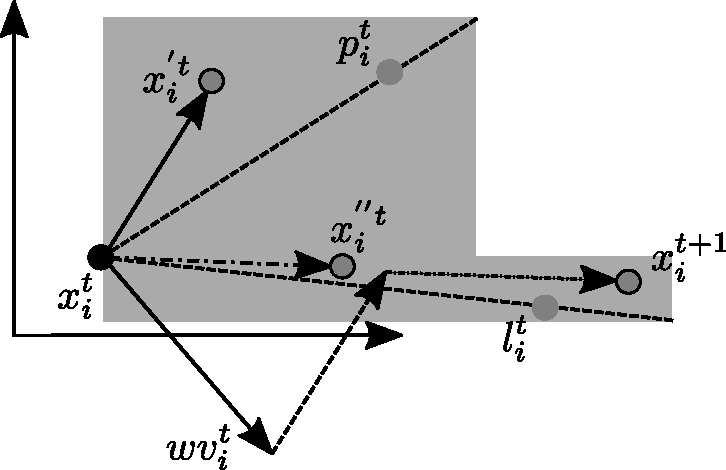
\includegraphics[width=0.60\textwidth]{"Part 2 - Search-Based Optimization/Particle Swarm Optimization/Images/SPSO2011-1.pdf"}
    \caption{Geometrical representation of standard PSO until 2007}
    \label{fig:STANDARDPSO_1}
\end{figure}


    
Figure~\ref{fig:STANDARDPSO_1} shows that each particle at each time step gets its distribution of all nearby positions and which is also a combination of two rectangles $D$ with sides parallel to the axes, with uniform probability distribution within each rectangle. In contrast, the variant proposed in 2011~\cite{clerc2012beyond} suggests the idea of an adaptive random topology in terms of communication between search agents and exploits the idea of rotational invariance (see Fig.~\ref{fig:STANDARDPSO}).


\begin{figure} [H]
\centering
    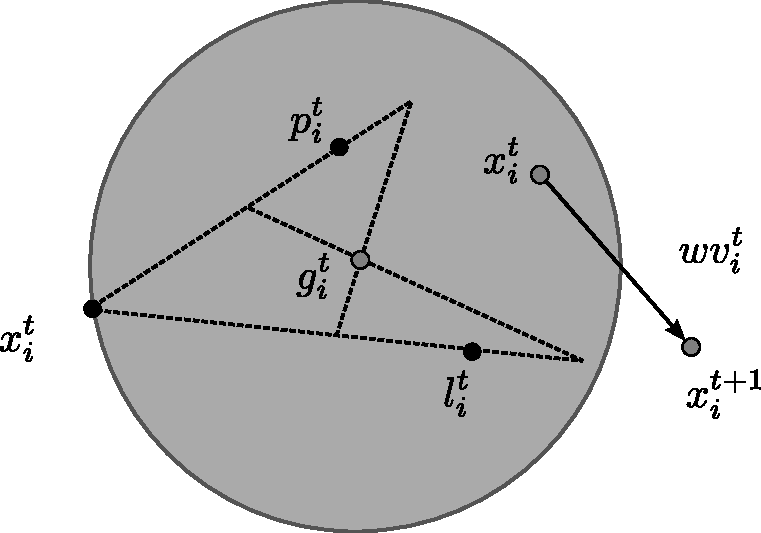
\includegraphics[width=0.60\textwidth]{"Part 2 - Search-Based Optimization/Particle Swarm Optimization/Images/SPSO2011.pdf"}
    \caption{Geometrical representation of standard PSO}
    \label{fig:STANDARDPSO}
\end{figure}



For each particle $i$ and at each time stage $t$, a center of gravity ${\vec{g}}_i^t$ is defined around three points:

\begin{itemize}
    \item The current position~(${\vec{x}}_i^t$)
    \item Point a little “beyond” the best previous personal position~(${\vec{p}}_i^t$) defined as:
    
    \begin{equation}\label{eq:bestpreviouspersonal position}
        {\vec{p}}_i^t={\vec{x}}_i^t+\ c_1{\vec{r}}1^t\otimes(\ {\vec{lB}}_i^t\ - {\vec{x}}_i^t)
    \end{equation}
    
    \item Point a little “beyond” the best previous position in the neighborhood~($ {\vec{l}}_i^t$) defined as:

      \begin{equation}\label{eq:best previous position in the neighbourhood}
        {\vec{l}}_i^t={\vec{x}}_i^t+\ c_2{\vec{r}}2^t\otimes(\ {\vec{gB}}^t\ - {\vec{x}}_i^t)
    \end{equation}
    
    \item Center of gravity(${\vec{g}}_i^t$) finally defined as:
    
    \begin{equation}\label{eq:gravitycentre}
        {\vec{g}}_i^t=\frac{\left({\vec{x}}_i^t+{\vec{p}}_i^t+{\vec{l}}_i^t\right)}{3}
    \end{equation}
    
\end{itemize}


In the case of Fig.~\ref{fig:STANDARDPSO} the $distribution~of~all~possible~next~positions$ (DNPP) obtained is a D-dimensional sphere defined as $\mathcal{H}_i({\vec{g}}_i^t, ||\vec{g}_i^t,\vec{x}_i^t||$), which is rotational invariant about its center, i.e., it does not change when the function is rotated.\\
In SPSO-2011, velocity is updated as follows:


\begin{equation}
       {\vec{v}}_i^{t+1}=w{\vec{v}}_i^t{+\mathcal{H}}_i({\vec{g}}_i^t,||\vec{g}_i^t - \vec{x}_i^t||)-\ {\vec{x}}_i^t
\end{equation}


While particle position is updated following Eq.~\eqref{eq:equation3}.

\subsubsection{Fully-informed PSO}

Human social behaviors inspired the authors to conclude that individuals are not influenced by a single individual but by those around them. Based on observations, they proposed a modification of the velocity equation of the canonical version of PSO~\cite{kennedy1995particle} with the purpose that each particle is influenced by the performance of all its neighbors and not by the performance of a single individual. The equations for the update of velocity and position are defined as: 

\begin{equation}\label{eq:speedwithneighbors}
      \vec{v}_i^{t+1}=w\vec{v}_i^t+\sum_{m=1}^{\left|C_i\right|}{\gamma_m^t\frac{(\mathcal{Y}_m^t-x_i^t)}{\left|C_i\right|}}
\end{equation}

\begin{equation}
       \vec{x}_i^{t+1}=\vec{x}_i^t +\ \vec{v}_i^{t+1}
\end{equation}


Inspired by the fact that an individual is influenced by the behavior of the individuals around him, the authors define the Eq.~\ref{eq:speedwithneighbors}. Where $C_i$ is the set of particles in the neighborhood of $i$, and $\gamma_m^t[0, c_1+\ c_2]^j$, where $c_1$ and $c_2$ are the learning coefficients, $j$ is the dimensionality of the problem and the position $\mathcal{Y}_m^t$ represents the best position that particle $m$ has visited until iteration $t$ (a particle that has obtained the best evaluation of the objective function).
The main contribution of this algorithm published in $2004$ that makes it different from other variants is the type of topology used in its particles~\cite{mendes2004population}. Since they all have the exact source of information, there is no difference in the amount of information shared. Some of the topologies that can affect or improve the performance of PSO are the following:

\begin{itemize}
    \item \textit{Ring}:
      this topology has a network configuration where the particle connections create a circular trajectory. Each particle in the network is fully connected to two others, thus forming a single continuous route, resulting in a ring structure as illustrated in Fig.~\ref{fig:ringtopology}. The algorithm that results from this topology is called Lbest PSO; in addition, such a topology can be generalized to a network structure in which neighborhoods of larger size are used.
    \item \textit{Star}:
    this social topology is shown in Fig.~\ref{fig:startopology}. Here, it is observed that all the particles in the swarm are interconnected. A PSO using the star topology is commonly named the Gbest PSO . The original implementation of the PSO used the star topology~\cite{kennedy1995particle}.
    \item \textit{Von Neumann}:
    this topology is a square grid where each particle has four neighbors. The 2-D variant is represented in Fig.~\ref{fig:squaretopology}, and the 3-D variant is represented in Fig.~\ref{fig:cubetopology}. This class of topologies allows the communication between the particles to be unusual and different from other social communication topologies.
\end{itemize}

\begin{figure}[H]\centering
  \begin{subfigure}[b]{0.23\textwidth}
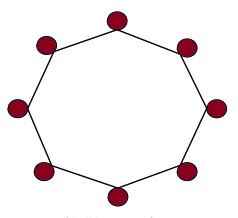
\includegraphics[width=\textwidth]{"Part 2 - Search-Based Optimization/Particle Swarm Optimization/Images/RING.jpg"}
    \caption{Ring.}
    \label{fig:ringtopology}
  \end{subfigure}
 \hfill
  \begin{subfigure}[b]{0.23\textwidth}
    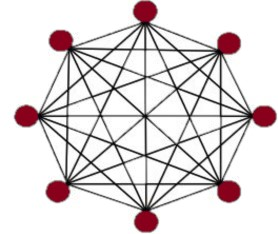
\includegraphics[width=\textwidth]{"Part 2 - Search-Based Optimization/Particle Swarm Optimization/Images/STAR.jpg"}
    \caption{Star.}
    \label{fig:startopology}
  \end{subfigure}
  \hfill
  \begin{subfigure}[b]{0.23\textwidth}
    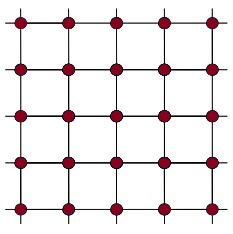
\includegraphics[width=\textwidth]{"Part 2 - Search-Based Optimization/Particle Swarm Optimization/Images/SQUARE.jpg"}
    \caption{Square.}
    \label{fig:squaretopology}
  \end{subfigure}
  \hfill
  \begin{subfigure}[b]{0.23\textwidth}
    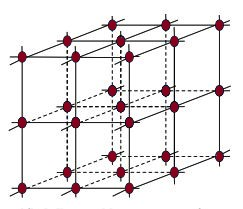
\includegraphics[width=\textwidth]{"Part 2 - Search-Based Optimization/Particle Swarm Optimization/Images/CUBE.jpg"}
    \caption{Cube.}
    \label{fig:cubetopology}
  \end{subfigure}
\caption{Social topologies}
  \label{fig:topologies}
\end{figure}

\subsubsection{Comprehensive Learning PSO}


The main novelty of this algorithm is that the authors propose a new function for updating the particle velocity defined as:

\begin{equation}
     \vec{v}_{i,j}=w\ast \vec{v}_{i,j} + c \ast {\vec{r1}_{i,j}} \ast \left ( \vec{lB}_{f_i(j),j} - \vec{x}_{i,j} \right ) 
\end{equation}


Where $fi=[f_i(1),f_i(2),\cdots,f_i(D)]$ defines which particles of $lB$ the particle $i$ should follow, and $D$ represent the dimensions of the problem. $lB_{f_i(j),j}$ can be any particle’s $lB$ including its own $lB$. The decision depends on probability $P_c$, referred to as the learning probability, which can take different values for different particles.
For each dimension of particle $i$, the authors generate a random number. If this random number is higher than $P_{c_i}$, the corresponding dimension will learn from its own $lB$; otherwise, it will learn from another particle’s $lB$.The selection method used by the tournament and the main steps for selection are as follows:

\begin{itemize}
    \item First, two particles are chosen randomly from the population, except the particle with its updated velocity.
     \item The objective value of the two particles($lB$) is compared, and the best of these is selected. In CLPSO the objective value is defined as the higher, the better, which means that to solve minimization problems, use the negative values of the function as objective values.
      \item Finally, using the winning particle as an example for the next generations to learn from that dimension, if all individuals are their own $lB$, then a random dimension is chosen for the particles to learn from the best $lB$ particles working on it.
\end{itemize}

\subsubsection{Fuzzy adaptative PSO} 

\paragraph{\textit{Fuzzy inference system}}

A fuzzy inference system is basically a conditional statements expressed of the form IF A THEN B, where A and B are labels of fuzzy sets defined by appropriated membership functions \cite{Zadeh1973}. A fuzzy inference system is composed of five functional blocks as can be seen in Fig.\ref{fig:FUZZY}:

\begin{figure}[h!]
\centering
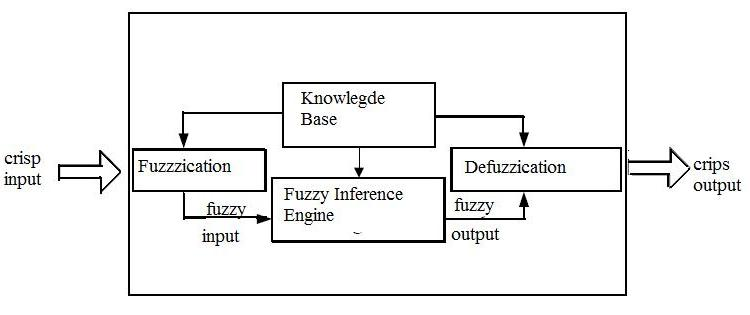
\includegraphics[width=0.90\textwidth]{"Part 2 - Search-Based Optimization/Particle Swarm Optimization/Images/Fig. 1.8.png"}
\caption{Fuzzy inference system}
\label{fig:FUZZY}
\end{figure}

\begin{itemize}
\item A \textit{rule base} containing a number of fuzzy if-then rules.
\item A \textit{database} which defines the memebership functions of the fuzzy sets used in the fuzzy rules.
\item A \textit{decision-making unit} which performs the inference operations on the rules.
\item A \textit{fuzzification interface} that transforms the crisp inputs into degrees of match with linguistic values.
\item A defuzzification interface which transforms the fuzzy results of the inference into a crisp output.
\end{itemize}

For more information about this computational area, the reader is advised to refer to the following references \cite{Sugeno1985,Jang1993}.\\

The authors of this paper, published in 2001~\cite{shi2001fuzzy} proposed to adapt the $PSO$ at four different levels: environment, population, individual, and component level. As mentioned above, the inertia weight is an important parameter in PSO, since it affect the convergence and exploration- exploitation trade-off in PSO process. As the inertia weight is a global variable, it can be applied to the whole population. A fuzzy system is basically an environment composed by if-then rules that determine the operation of the environment \cite{shi2001fuzzy}. The authors designed a fuzzy system to adapt the inertia weight dynamically. Typically, the system's inputs are variables that measure the performance of the $PSO$, and the output is the inertia weight or the change in the inertia weight. The current best performance evaluation named $CBPE$ indicates the best solution found by the $PSO$. Due to the wide variety of optimization problems, this term must be converted into a normalized format called $NCPBE$. Assume that to solve a minimization problem and the actual minimum is denoted $CBPE_{min}$ and the non-optimal $CBPE$ is denoted $CBPE_{max}$, which represents any suboptimal solution that is equal to or greater than $CBPE_{max}$. The normalized $CBPE$ ($NCBPE$) can be computed as three fuzzy variables in order to define three fuzzy sets: low, medium, and high with associated membership functions as $left\_triangle$, $triangle$ and $right\_triangle$, respectively. The definitions of these three membership functions are: 

\begin{equation}
    f_{left\_triangle}=
    \begin{cases}
    1 & \text{if $x < x_1$}\\
    \frac{x_2 -x}{x_2 -x_1} & \text{if $x_1 \leq x \leq x_2$}\\
    0 & \text{if $x > x_2$}
    \end{cases}
\end{equation}

\begin{equation}
    f_{triangle}= \begin{cases}
    0 & \text{if $x<x_1$}\\
    2 \frac{x - x_1}{x_2 -x_1} & \text{if $x_1 \leq x \leq \frac{x_2 +x_1}{2}$}\\
    2 \frac{x_2 -x}{x_2 -x_1} & \text{if $\frac{x_2 +x_1}{2} < x \leq x_2$}\\
    0 & \text{if $x > x_2$}
    \end{cases}
\end{equation}

\begin{equation}
    f_{right\_triangle} = \begin{cases}
    0 & \text{if $x < x_1$}\\
    \frac{x -x_1}{x_2 -x_1} & \text{if $x_1 \leq x \leq x_2$}\\
    1 & \text{if $x > x_2$}
    \end{cases}
\end{equation}

where $x_1$ and $x_2$ are critical parameters that determine the shape and location of the functions, other definitions of membership functions are possible, of course. However, the authors have found that the ones they propose are useful for various problems and easy to implement on microcontrollers and microprocessors.

\subsection{Major PSO variants for multi-objective optimization}
\label{sec:variants2}

PSO is a powerful tool for solving single-objective problems; for that reason, researchers expanded its capabilities to the multi-objective domain. The idea is to generate PSO-based approaches that can optimize more than one objective function. Multi-objective optimization (MO) is related to problems that are necessary to search for solutions for conflicting goals. The main difference between MO and single-objective optimization is that in MO, a set of solutions called a Pareto front is generated where each objective value is a feasible solution \cite{coello2007evolutionary}. This section briefly discusses the most relevant versions of the PSO for MO problems. These variants were selected based on their citations in scientific repositories.

\subsubsection{MOPSO} 

This algorithm proposed in 2002 introduces concepts of multiobjective optimization to modify the original PSO algorithm and implement it to solve multiobjective optimization problems, the authors named this approach multiobjective particle swarm optimization (MOPSO)~\cite{coello2002mopso} and was validated with algorithms such as Pareto Archived Evolution Strategy (PAES)~\cite{knowles1999pareto} and the Non-dominated Sorting Genetic Algorithm II (NSGA II)~\cite{deb2000fast}.

\paragraph{\textit{Algorithm design and general structure}}

The analogy of the particle swarm with evolutionary algorithms made it evident that this algorithm could be designed for a multi-objective approach. Introducing concepts such as the Pareto front and using a memory known as a global repository in which each particle will deposit its flight experiences after each cycle to establish dominance degrees.
Another adapted mechanism was that each particle could choose a different leader to perform the search and is based on the generation of hyper-cubes, which allows dividing the search space into already explored spaces; the general structure of the algorithm is listed below:

\begin{enumerate}
    \item Initialize population with random position and velocity vectors
    \item Evaluate the objective value of each particle in the set of objective functions, with their respective constraints and bounds $lb$ and $ub$ using the Eq.~\ref{eq:mo_criterion}.
    \item Archive=non-dominated solutions.
    \item Determine the objective value of each particle.
    \item Apply the Eq.~\ref{eq:equation2} and~\ref{eq:equation3}.
    \item Update personal best and the archive
    \item Repeat steps 5 to 7 until the stop criterion is reached.
\end{enumerate}

\begin{equation}
\begin{split}\label{eq:mo_criterion}
    \text{Minimize/Maximize } f_n (x) &,\quad n=\{1,2,\cdots,O\}\\
    \text{Subject to } g_j(x) \geq &, \quad j = \{1,2,\cdots,J\}\\
    h_k(x)=0 &, \quad k=\{1,2,\cdots,K\}\\
    x_i^{(lb)} \leq x_i \leq x_i^{(ub)} &, \quad i=\{1,2,\cdots,N\}
\end{split}
\end{equation} 


In MOPSO the velocity and position update equations remain the same as Eq.~\eqref{eq:equation2} and Eq.~\eqref{eq:equation3} of PSO. All the stated parameters are also the same except the objective function. The objective function contains multiple objectives as formulated in Eq.~\eqref{eq:mo_criterion}.
This multi-objective algorithm has been widely used in the literature for applications in different fields; three of the most notable fields, according to the reports in~\cite{lalwani2013comprehensive} are Electrical Engineering, Industrial Engineering, Flow-shop, and Job-shop Scheduling.

\subsubsection{SMPSO}

In 2009, Nebro et al.~\cite{nebro2009smpso} studied six representative variants of MOPSO and found that they had problems solving multi-modal problems, it meas those problems with two or more feasible solutions. The problem was the "swarm explosion"~\cite{clerc2002particle}: erratic movements toward the upper and lower boundaries of particle positions that occur when particles acquire very high velocity. Based on a MOPSO algorithm, they presented in~\cite{nebro2009smpso} a new multi-objective PSO algorithm using the velocity constraint strategy~\cite{clerc2002particle}. Their proposal could obtain proper particle positions when high velocity was present, avoiding the swarm explosion effect. The new algorithm, called Speed-constrained Multi-objective PSO (SMPSO), applies the following equations to perform its task:

\begin{equation} \label{eq:con_coe}
\chi = \frac{2}{2 -\varphi - \sqrt{\varphi^2 -4\varphi}}
\end{equation}
where
\begin{equation}
\varphi = \left\{ \begin{matrix}
    C_1 +C_2 & \rm{if} \quad C_1 +C_2 > 4 \\ 
    1 & \rm{if} \quad C_1 +C_2 \leq 4
\end{matrix} \right.
\end{equation}
where $C_1$ and $C_2$ are the parameters to control the effect of the personal and global best particles.
Once the velocity of the particles is calculated in the original form ~\cite{nebro2009smpso} it is obtained the constriction coefficient through Eq.~\ref{eq:con_coe}. The calculated velocity is multiplied by the constriction coefficient, and then the velocity is constrained by Eq.~\ref{eq:vel_con} The effect of this calculation is to provide diversity to the solutions, otherwise the exploitation of the particles would be intensified.

\begin{equation} \label{eq:vel_con}
v_{i, j}^t = \left\{ \begin{matrix}
    \Delta b_j & {\rm if} \, v_{i,j}^t > \Delta b_j\\
    -\Delta b_j & {\rm if} \, v_{i,j}^t \leq -\Delta b_j\\
    v_{i,j}^t & {\rm otherwise}
\end{matrix} \right.
\end{equation}
where
\begin{equation}
    \Delta b_j = \frac{(ub_j -lb_j)}{2}
\end{equation}
where $ub$ and $lb$ are the upper and lower boundaries of search space, and $\Delta b_j$ is the center point between them.
By implementing this strategy, SMPSO overcomes the swarm explosion effect of MOPSO algorithms. They reported that the approximations to the Pareto front found by their algorithm were better than the MOPSO algorithms. The SMPSO was the fastest algorithm converged to the Pareto front in their experiments.

\subsubsection{FC-MOPSO}

This algorithm presented in 2017~\cite{mokarram2018new} proposes a new multi-objective algorithm, originally targeted at the problem of optimal design of engineering problems with few function evaluations.\\
The main contributions are the following:
\begin{itemize}
    \item Effective leader selection process for each particle to guarantee diversity and fast convergence.
    \item The FC-MOPSO is a modified algorithm for handling discrete optimization problems.
    \item Use of constant value close to unity: $\alpha = 0.9.$.
\end{itemize}
In the original PSO $\vec{lB}_i^t$ represents the best position found by the $i^{th}$ particle in the $t^{th}$ iteration. However, in a multi-objective problem the authors generalize this concept to the set $P_i$, which is defined as the set of non-dominant solutions found so far by the particle $i$. Subsequently a particle called $\vec{psel}_i$ will be selected from $P_i$ for the flight stage. In the same way the concept $\vec{gB}_i$ is generalized to $\vec{Leader}_i$ which randomly selects $n$ neighboring sets $P_j (j\in[1,...,n])$ by extracting non-dominant sets to assign to $Q_i$. A non-dominant set means a group of particles of the population, that have noncompetitive objective values and that do not benefit the search for the global optimum.

\begin{equation}
    v_{i,j}^{t+1} \leftarrow \left\{  \begin{matrix} v_{i,j}^{t+1} & \rm{ if} \, |v_{i,j}^{t+1}| \leq v_m^k \\ v_m^k sign ( v_{i,j}^{t+1} ) & \rm{otherwise} \end{matrix} \right. , k \in [1, \cdots,s]
\end{equation}

Where $v_m = [v_m^1, \dots, v_m^s]$ is the vector of maximum admissible speeds. The authors suggest that FC-MOPSO starts with random velocities no greater than $v_{m} = 0.1(ub - lb)$, where $ub$ and $lb$ are the upper and the lower boundaries of the search space, respectively. In other words, they prevent the method from starting with large velocities while starting with some speeds to start the search at a more advanced stage. 

%lgorithms should use the package algorithmic. An example is given below:


%%%%%%%%%%%%%%%%%%%%%%%% ALGORITHM
%\begin{algorithm}[ht!]
	%\renewcommand{\baselinestretch}{0.8}
%	\caption{Example algorithm}
    
 %   Parameters: enter parameters here
    
  %  Output: enter output here.
    
%	\begin{algorithmic}[1] 
%		\STATE{Do this.}
		
%        \REPEAT
		
%		\FOR{each model $m$}
		
%		\STATE Do that.
				
%		\ENDFOR
%		\UNTIL the maximum number of iterations is reached
		
%	\end{algorithmic}
	
%\end{algorithm}
%%%%%%%%%%%%%%%%%%%%%%%% ALGORITHM

\section{PSO Applications} \label{sec:apps}

The applications presented were chosen based on the relevance of current works consulted in the $Google Scholar$ repositories.\\
In recent years, robotics has undergone significant development. The specialization of many tasks requires the optimization of execution times and precision in the robot's movements.
In this sense, the modeling parameters of the robot were explored in~\cite{bingul2011dynamic}, where the researchers used a combination of the Least Square (LS) method and PSO to estimate a robotic arm's inertia parameters. The estimation performed by the algorithm matches closely with the manufacturer-provided values.
The trajectory planning for mobile
robots through PSO was implemented by Abdalla et al.~\cite{abdalla2017mobile}, Zeng et al.~\cite{zeng2016path}, and Wang et al.~\cite{wang2015trajectory}. Zeng et al. used a PSO based on a non-homogeneous Markov chain and Differential Evolution algorithm to generate a path into a space with obstacles for intelligent robots. Abdalla et al. proposed a combination of the artificial potential field (APF) with fuzzy logic, where PSO was used to optimize the membership functions of the fuzzy controller to acquire the mobiles robot trajectory, and Wang et al. combined the PSO algorithm with kinematics equations to trajectory planning in the free-floating space robot, simulating a couple of a spacecraft and a manipulator robot.

Electrical energy has been studied for centuries, and its use has been extended to all possible areas in recent decades. Now, with the renewable production of electrical energy, it is imperative to optimize its use and its distribution and production for maximum utilization.
Electricity sometimes came from a cascade system of hydroelectric generators. Evaporation, irrigation systems, and other factors affect the water level in the reservoirs. Mahor and Saroj~\cite{mahor2012short} used a PSO based algorithm to optimize the generation schedule of a real system of hydroelectric cascade system in India.
In \cite{bahrami2014short} Bahrami et al. use the PSO algorithm to determine the optimal parameter in a grey model. This model brings the opportunity to forecast the electric load in the short term, using minimal historical data. The method was used to forecast the load in Iran and New York electrical networks.
In 2016, Mesbahi et al. used a hybrid PSO-Nelder-Mead algorithm to identify and model electric vehicle batteries and then used this information to simulate vehicle energy demand, which allows maximum energy harvesting~\cite{mesbahi2016dynamical}. Finally, Mesbahi et al. compare their results against the power consumption of a physical urban electric vehicle, with a modeling error inferior to 0.5\%.
Mozafar et al. applied a multiobjective algorithm, using PSO combined with GA to optimize the location and capacity of renewable power sources and electric vehicle charging stations within the same distribution network.~\cite{mozafar2017simultaneous}.

\section{Conclusions}
\label{sec:conclusions}

The PSO is an interesting algorithm that has attracted the attention of researchers and practitioners from different areas over the years. The simplicity of the PSO makes it a popular mechanism for single-objective optimization. Their operators are easy to implement and permit finding solutions to complex problems. Since the PSO has been extensively used, it has also been modified to improve its performance.
Multi-objective problems require more sophisticated algorithms that permit handle with them.
In this sense, the PSO has been extended for multi-objective optimization. Regarding the importance of the PSO, it is possible to see how this method stills being a source of research from different repositories. The multiple modifications of the PSO algorithm are an excellent example of this. This chapter just considered the most relevant derivative work of PSO from 2010 to 2020. There exists more, but analyzing them is a complex and irrelevant task to the present work scopes. The quantity of derivative works is similar to the number of applications of the PSO; since its implementation is relatively easy and the code is entirely available, it is possible to find a significant number of articles that reports result from different fields of applications. It is possible to conclude that the PSO is one of the most important meta-heuristic algorithms, and the research related to it is still has lots to promise.

\subsection{Exercises}
\label{sec:exeercises}

\begin{enumerate}
    \item Program the Rosenbrock function defined as follows:
    
    \begin{equation} \label{eq:rosen}
    f(x_1 \cdots x_n) = \sum_{i=1}^{n-1} (100(x_i^2 - x_{i+1})^2 + (1-x_i)^2)
\end{equation}

Where $-2.048 \leq x_i \leq 2.048$ and $\text{ the minimum at }f(1, 1, \cdots, 1) = 0$.  Once you have implemented the Rosenbrock function plot its surface in 2 dimensions.

    \item Considering the Rosenbrock function, initialize a random population of 50 particles and plot them in the the 2-dimensional surface of the function.
    
    \item Implement the standard version of the PSO explained in this chapter to minimize the Rosenbrock function. You need to obtain the curve of convergence of the best solution at each iteration and plot it.
    
    \item Implement a code of the Fully Informed PSO that was explained in this chapter. The Fully Informed PSO should be able to minimize the Rosenbrock function. Obtain the convergence curve and compare it with the one obtained by the standard PSO. 
    
\end{enumerate}

\subsection{Answers to the exercises}
\label{sec:answers}

\begin{enumerate}
    \item Rosenbrock function top view
    \begin{figure} [H]
    \centering
        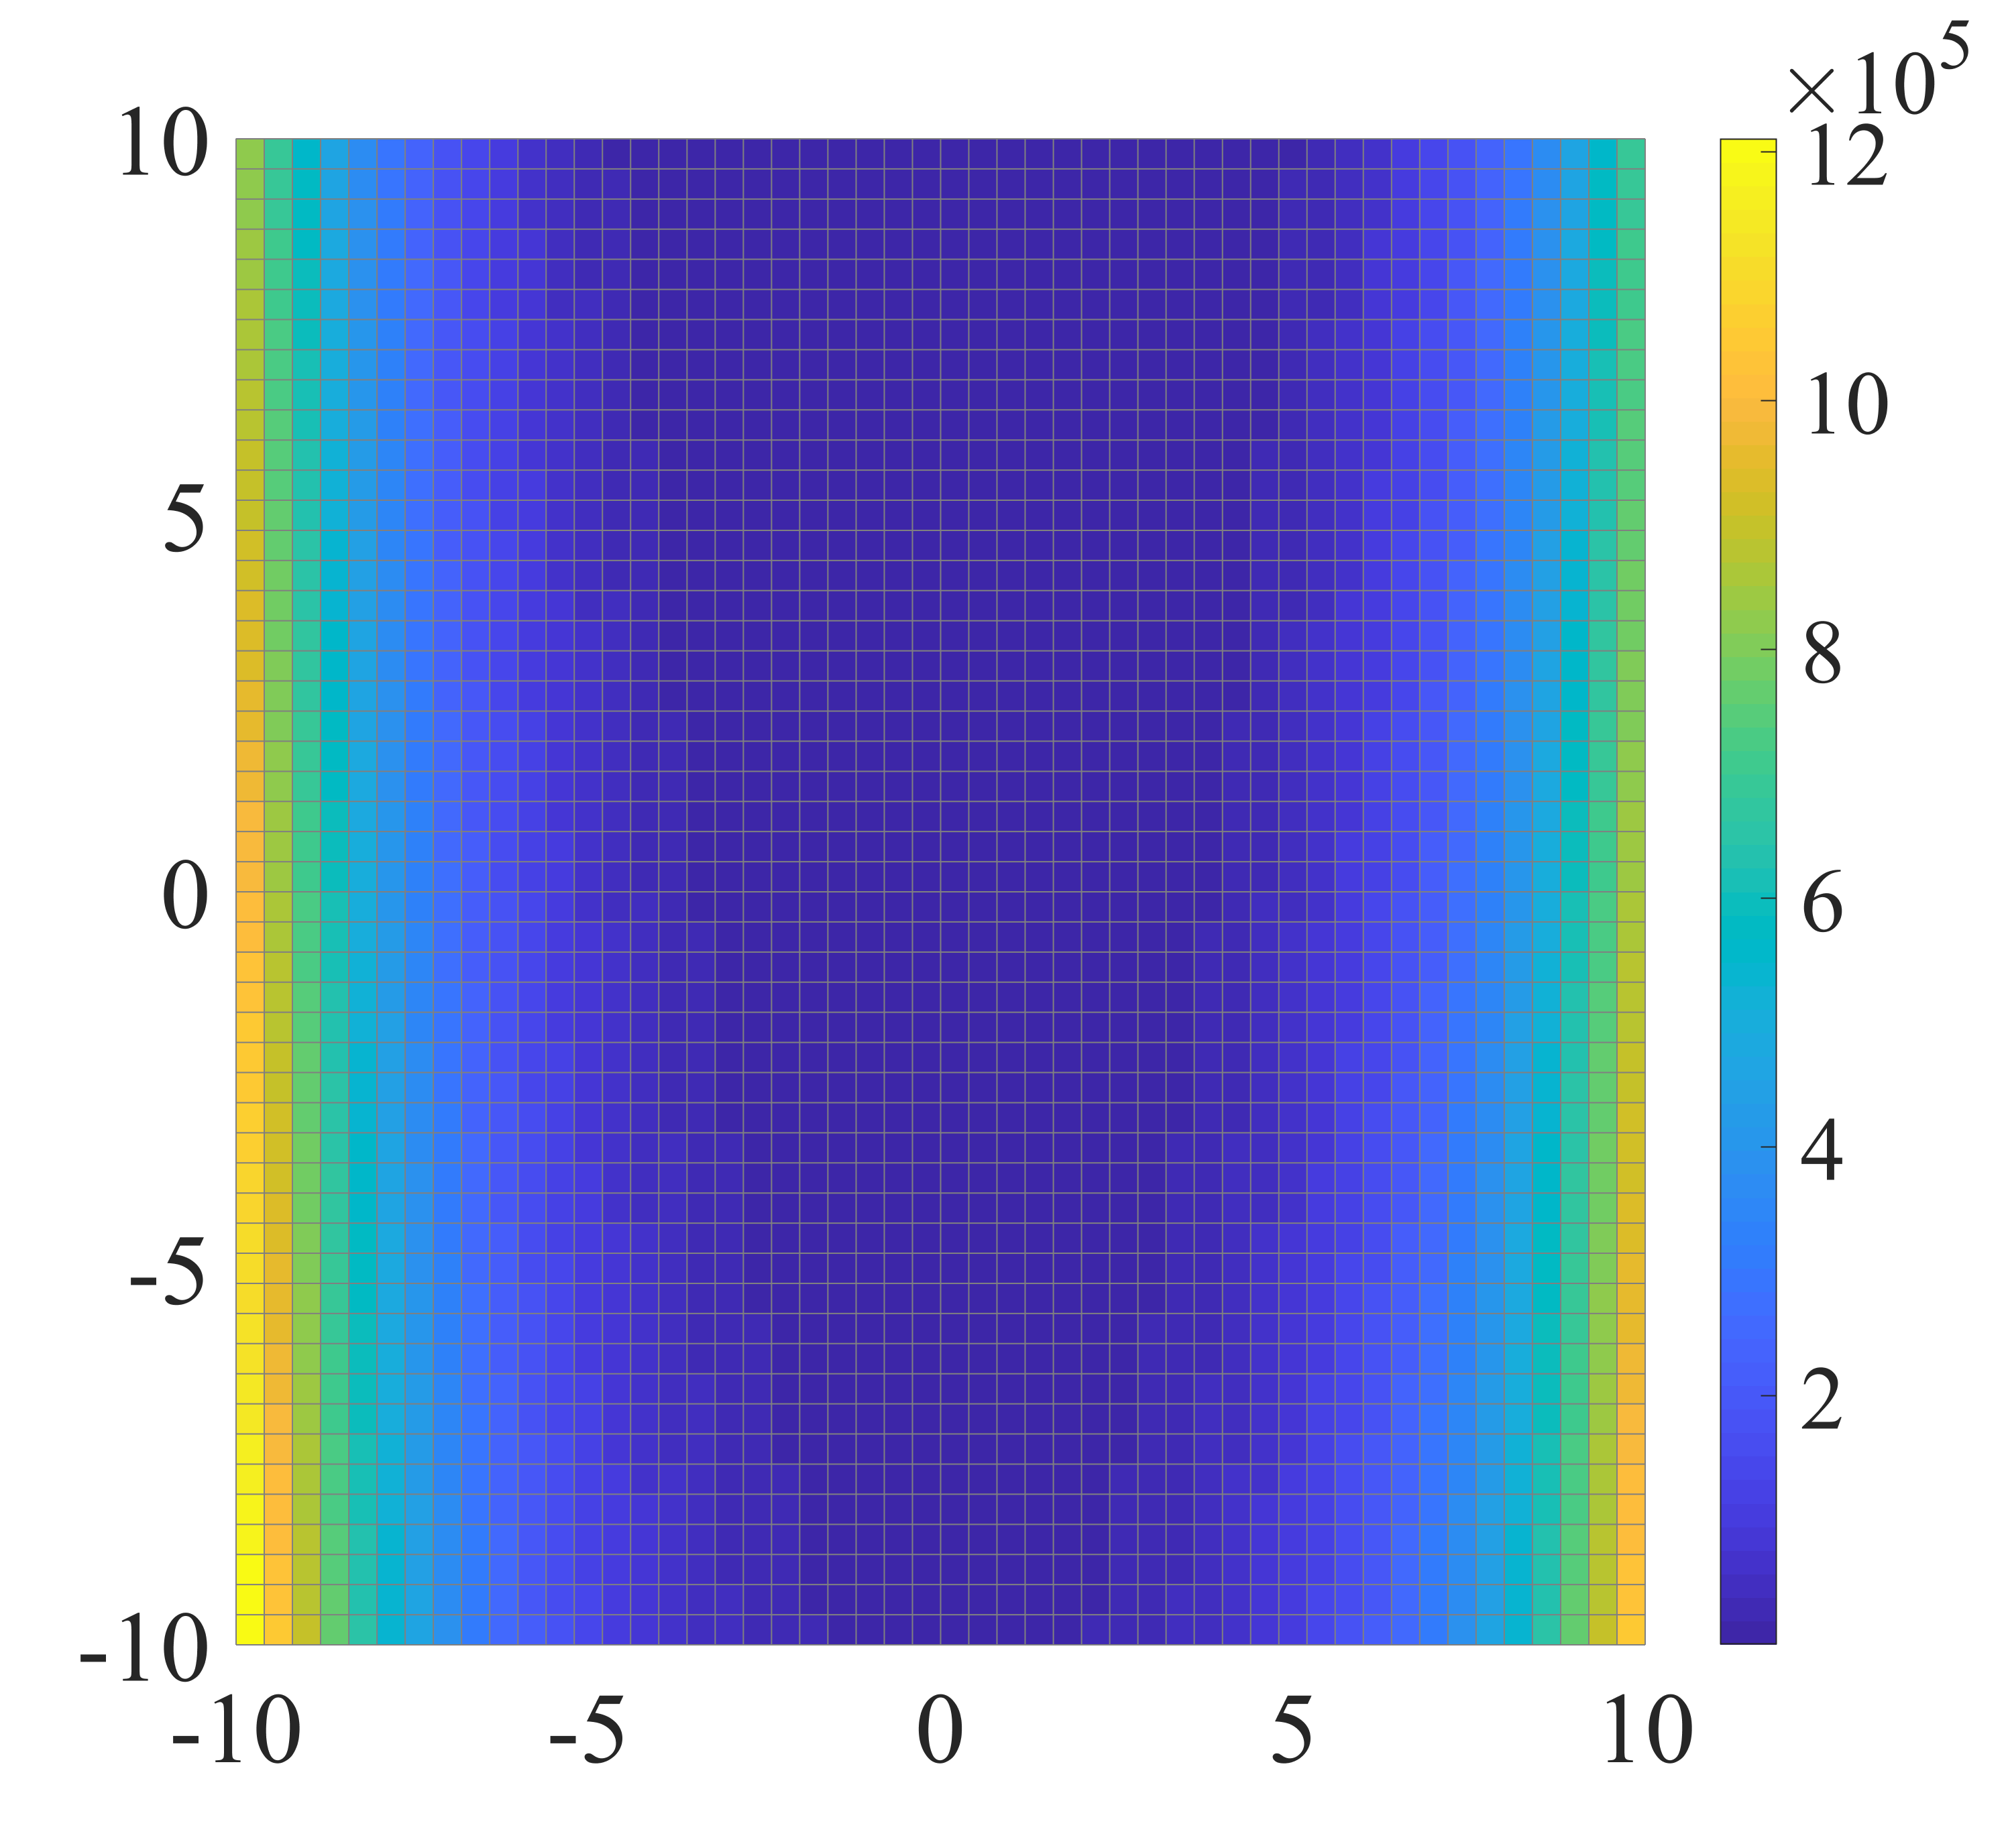
\includegraphics[width=0.60\textwidth]{"Part 2 - Search-Based Optimization/Particle Swarm Optimization/Images/rosenbrock.PNG"}
        \caption{Rosenbrock function}
        \label{fig:rosenbrock_function}
    \end{figure}
    
    \item initialization of a random population of 50 particles on the 2-dimensional surface of the Rosenbrock function.
    \begin{figure} [H]
    \centering
        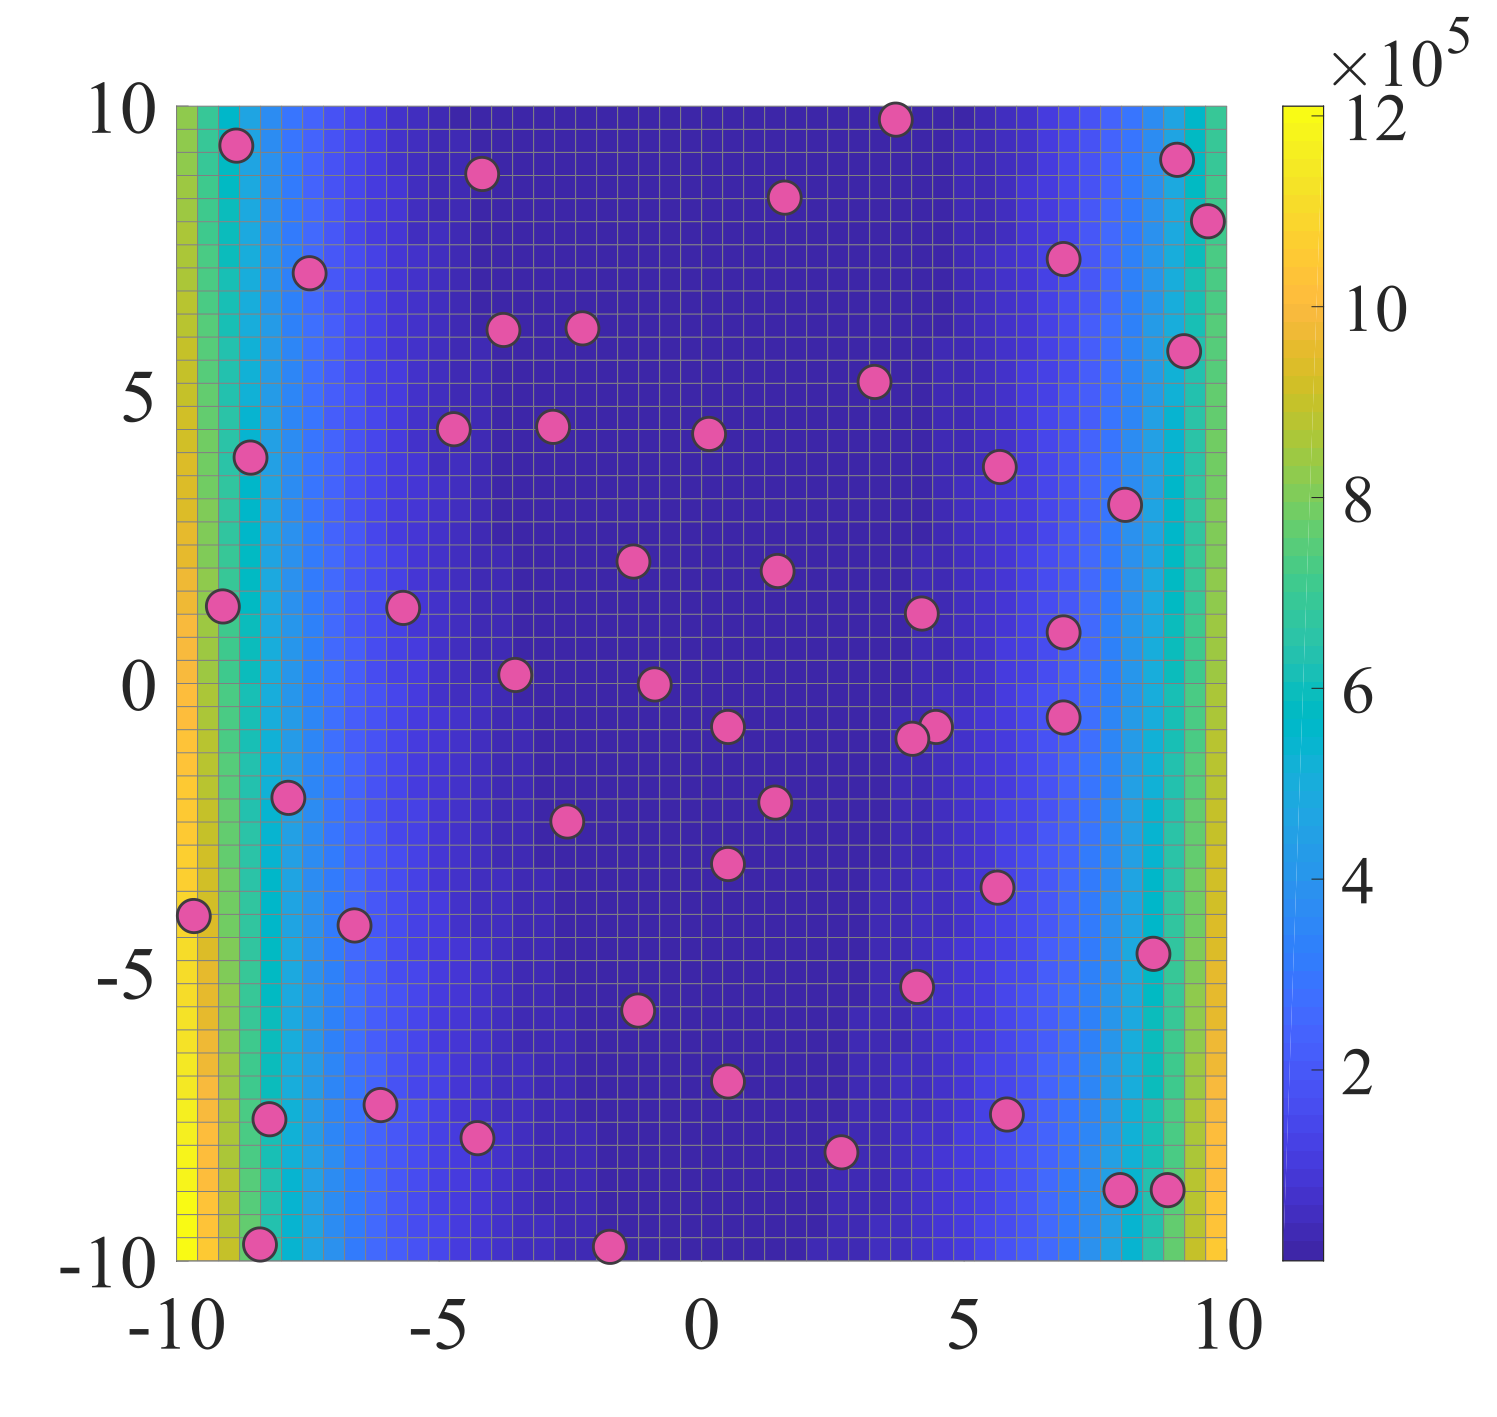
\includegraphics[width=0.60\textwidth]{"Part 2 - Search-Based Optimization/Particle Swarm Optimization/Images/rosenbrock_plot_particles.PNG"}
        \caption{Initialization of 50 particles on the Rosenbrock function}
        \label{fig:rosenbrock_function_inicializarion_particles}
    \end{figure}

    \item Convergence plot of standard particle swarm optimization version 
    
        \begin{figure} [H]
    \centering
        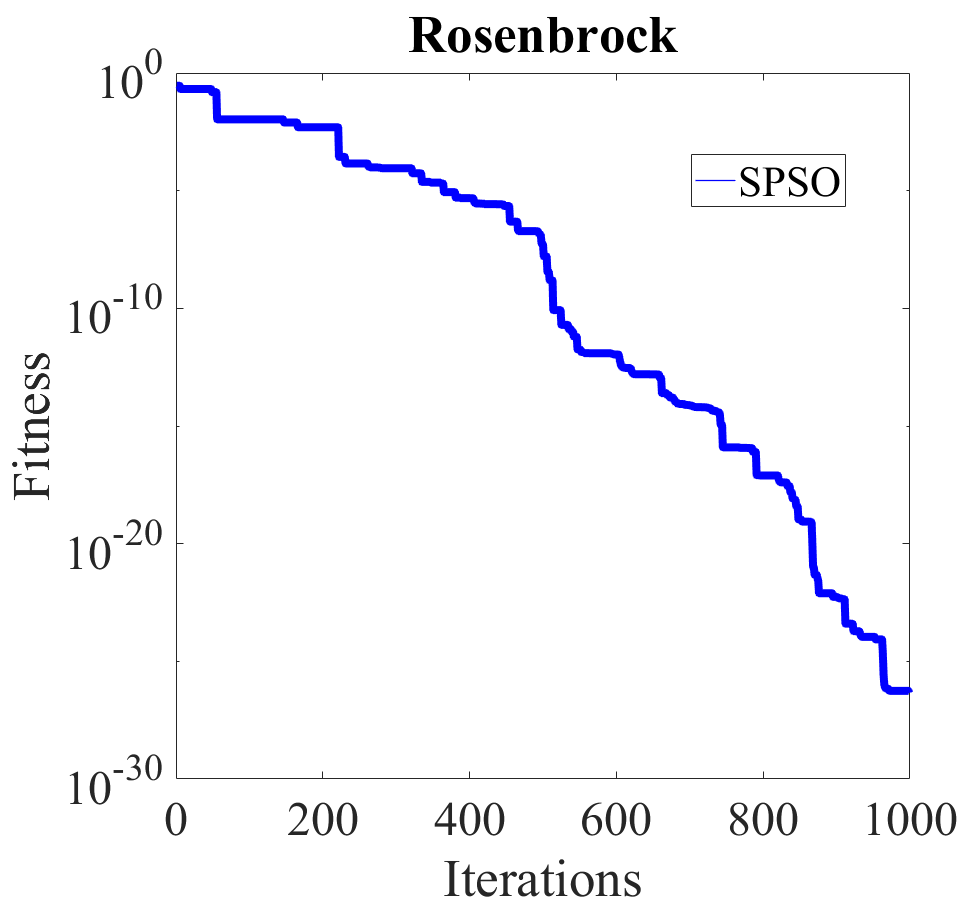
\includegraphics[width=0.60\textwidth]{"Part 2 - Search-Based Optimization/Particle Swarm Optimization/Images/SPSO.png"}
        \caption{SPSO convergence graph}
        \label{fig:SPSO_convergence_graph}
    \end{figure}
    
    \item Comparison of convergence plots between standard particle swarm optimization~(SPSO) and Fully informed Particle Swarm~(FIPS).
    
     \begin{figure} [H]
    \centering
        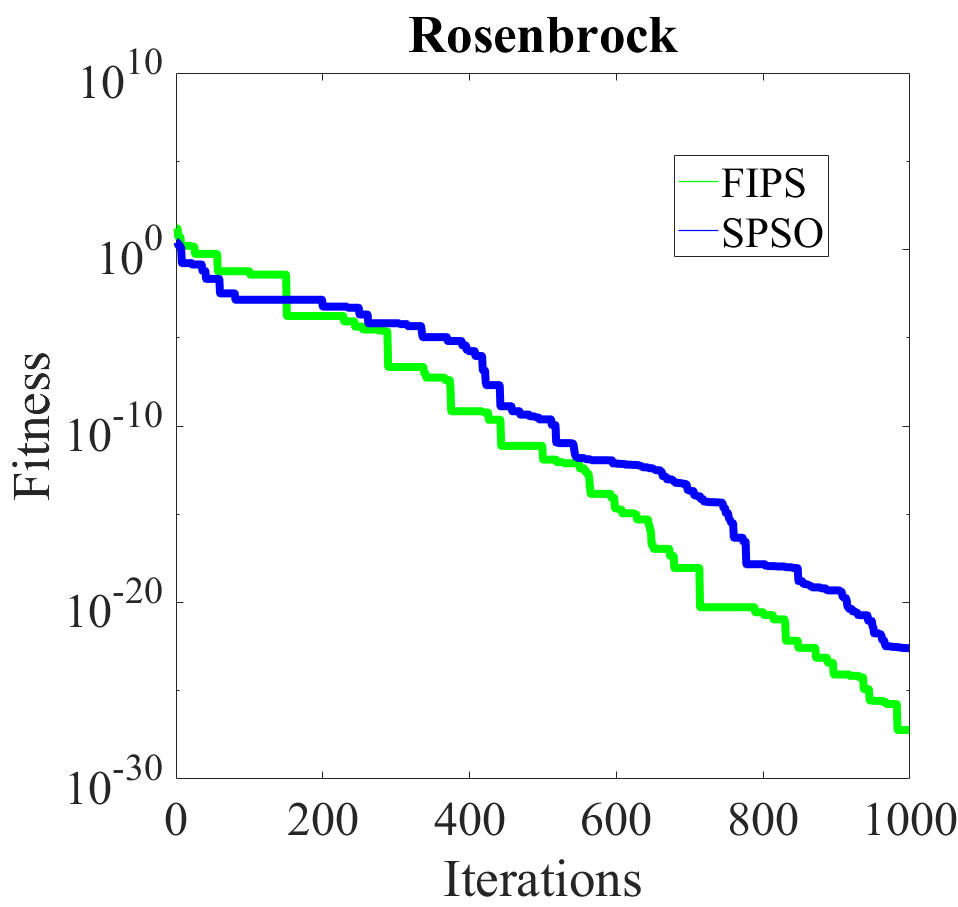
\includegraphics[width=0.60\textwidth]{"Part 2 - Search-Based Optimization/Particle Swarm Optimization/Images/VersusPS.png"}
        \caption{SPSO vs. FIPS convergence plots}
        \label{fig:SPSOvs.FIPS_convergence_plots}
    \end{figure}
    
\end{enumerate}



\bibliographystyle{unsrt}
\bibliography{bibliography}
